
% Primer bloque de figuras
\begin{figure}[H]
\centering
\begin{subfigure}[b]{0.49\textwidth}
	\centering
	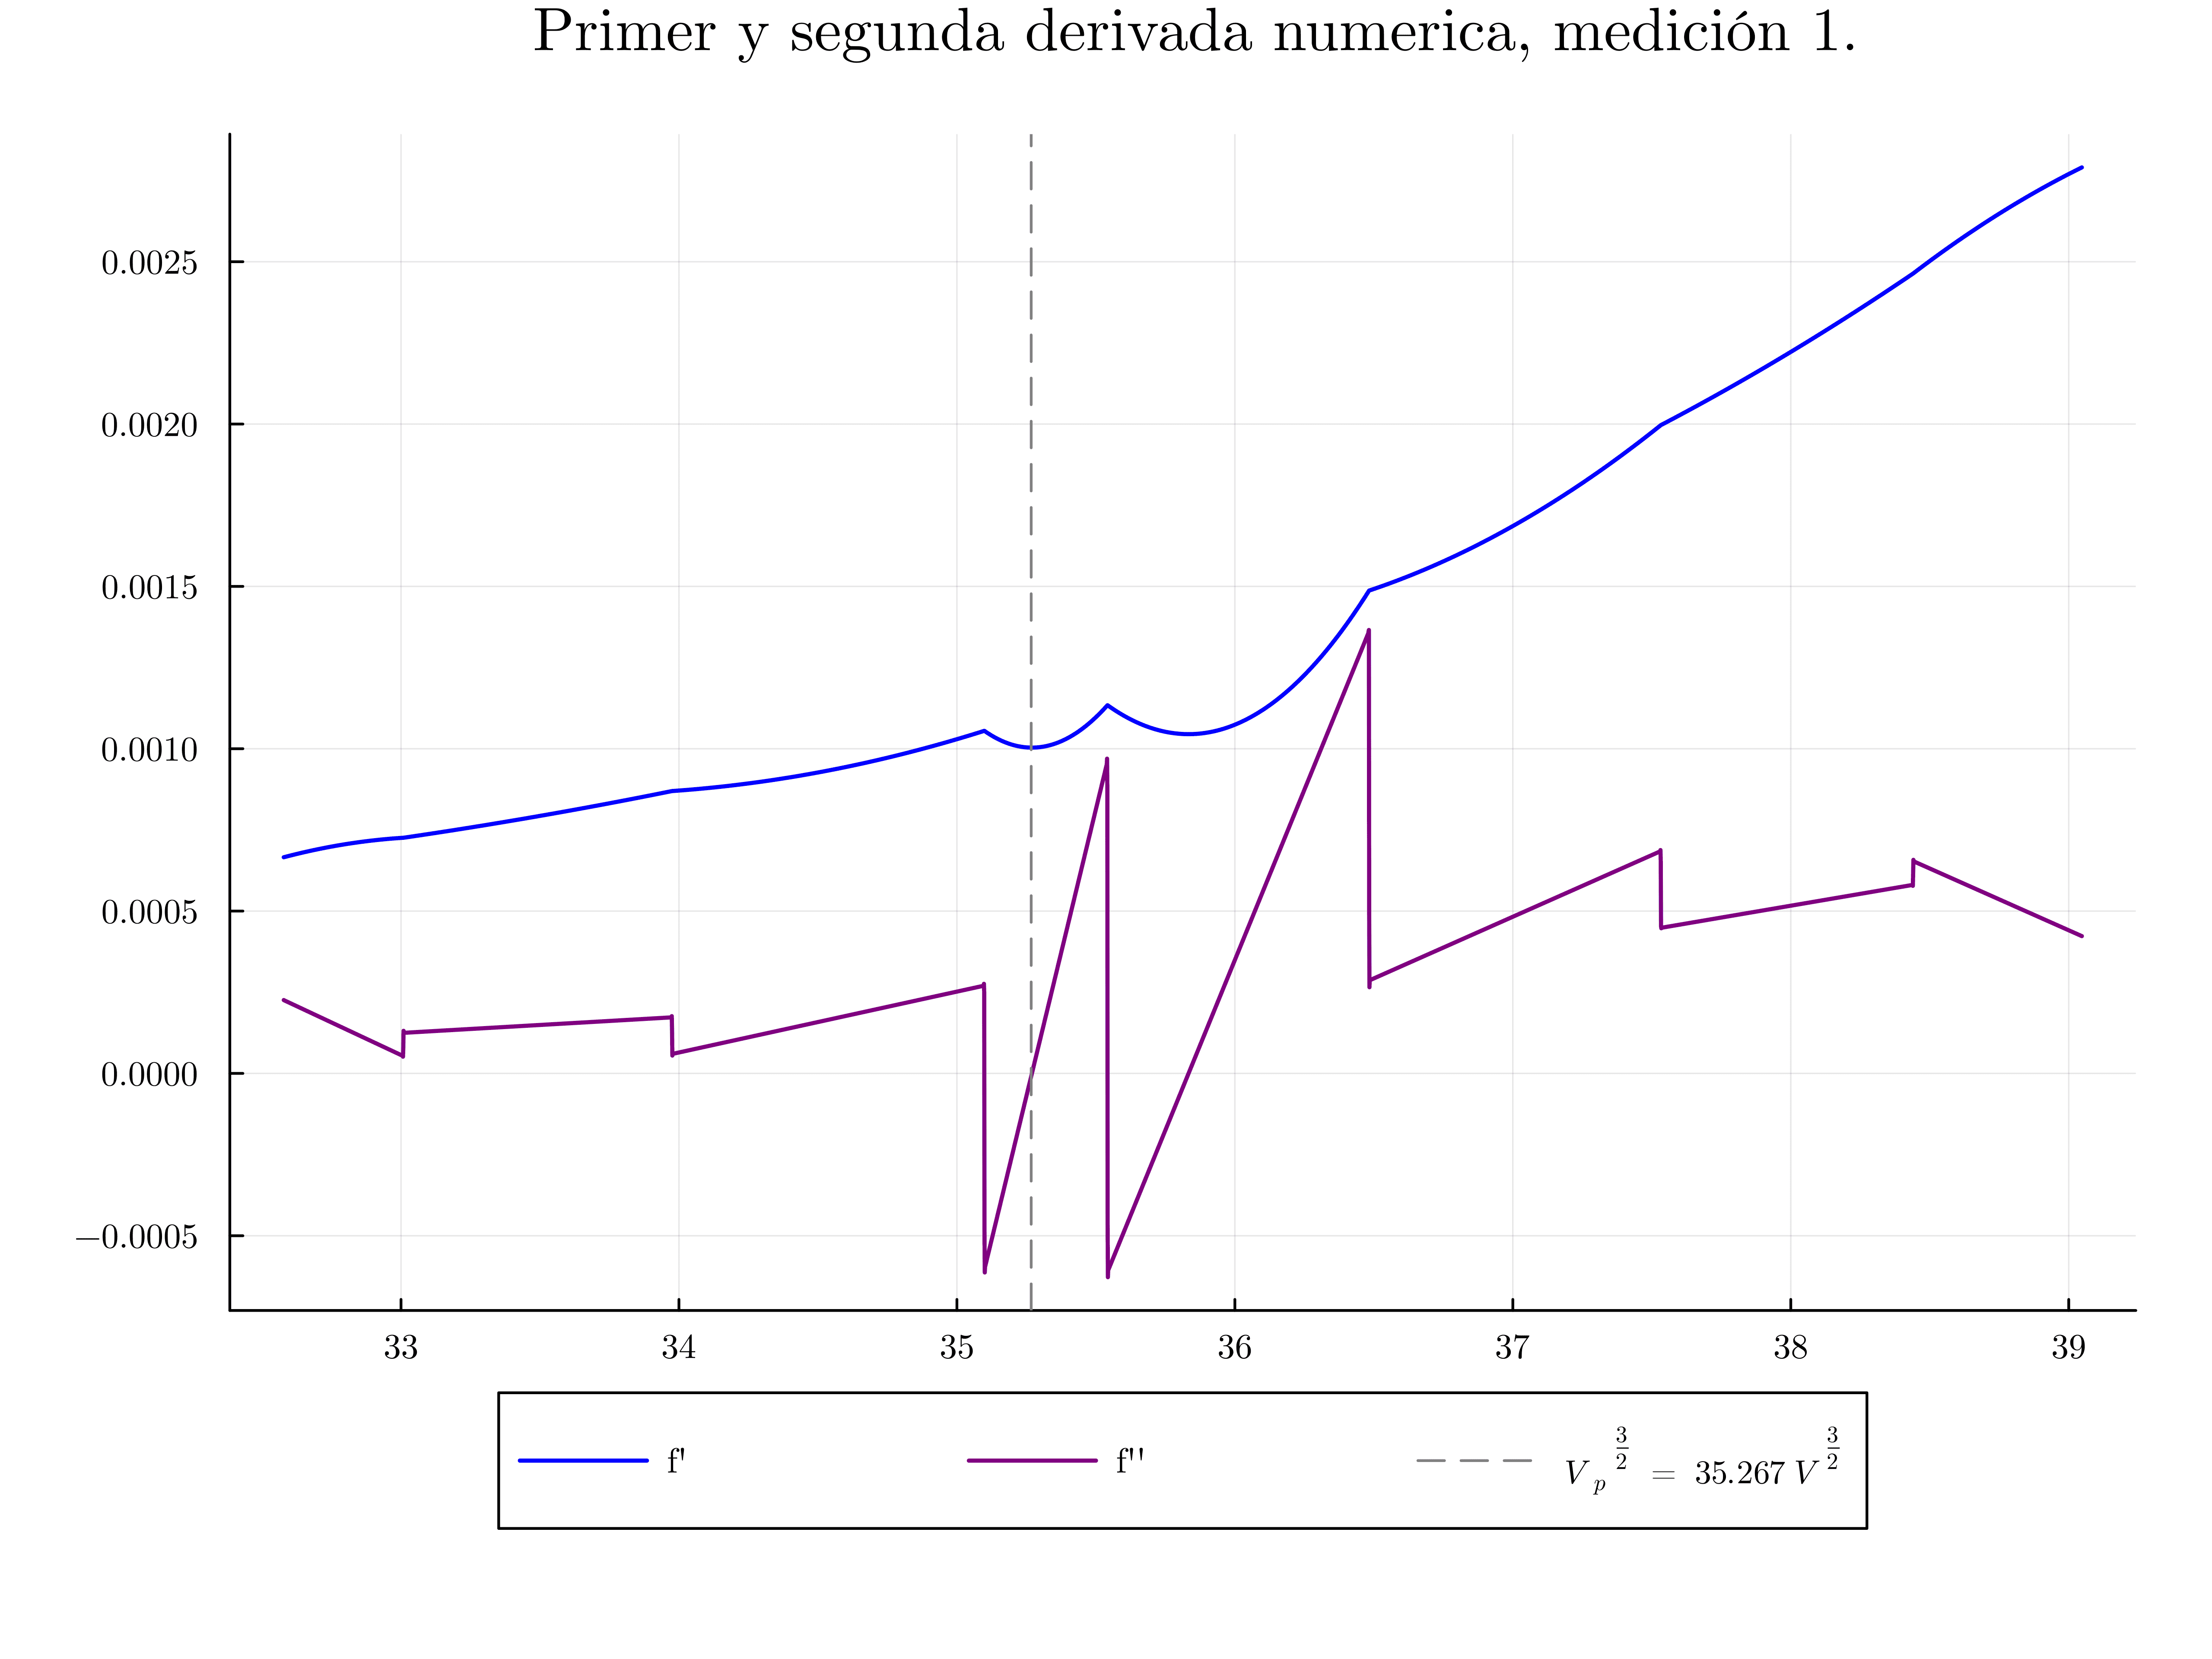
\includegraphics[width=\linewidth]{img/potderps1.png}
	\caption{Barrido n°: 1}
	\label{fig:potderps1}
\end{subfigure}
\hfill
\begin{subfigure}[b]{0.49\textwidth}
	\centering
	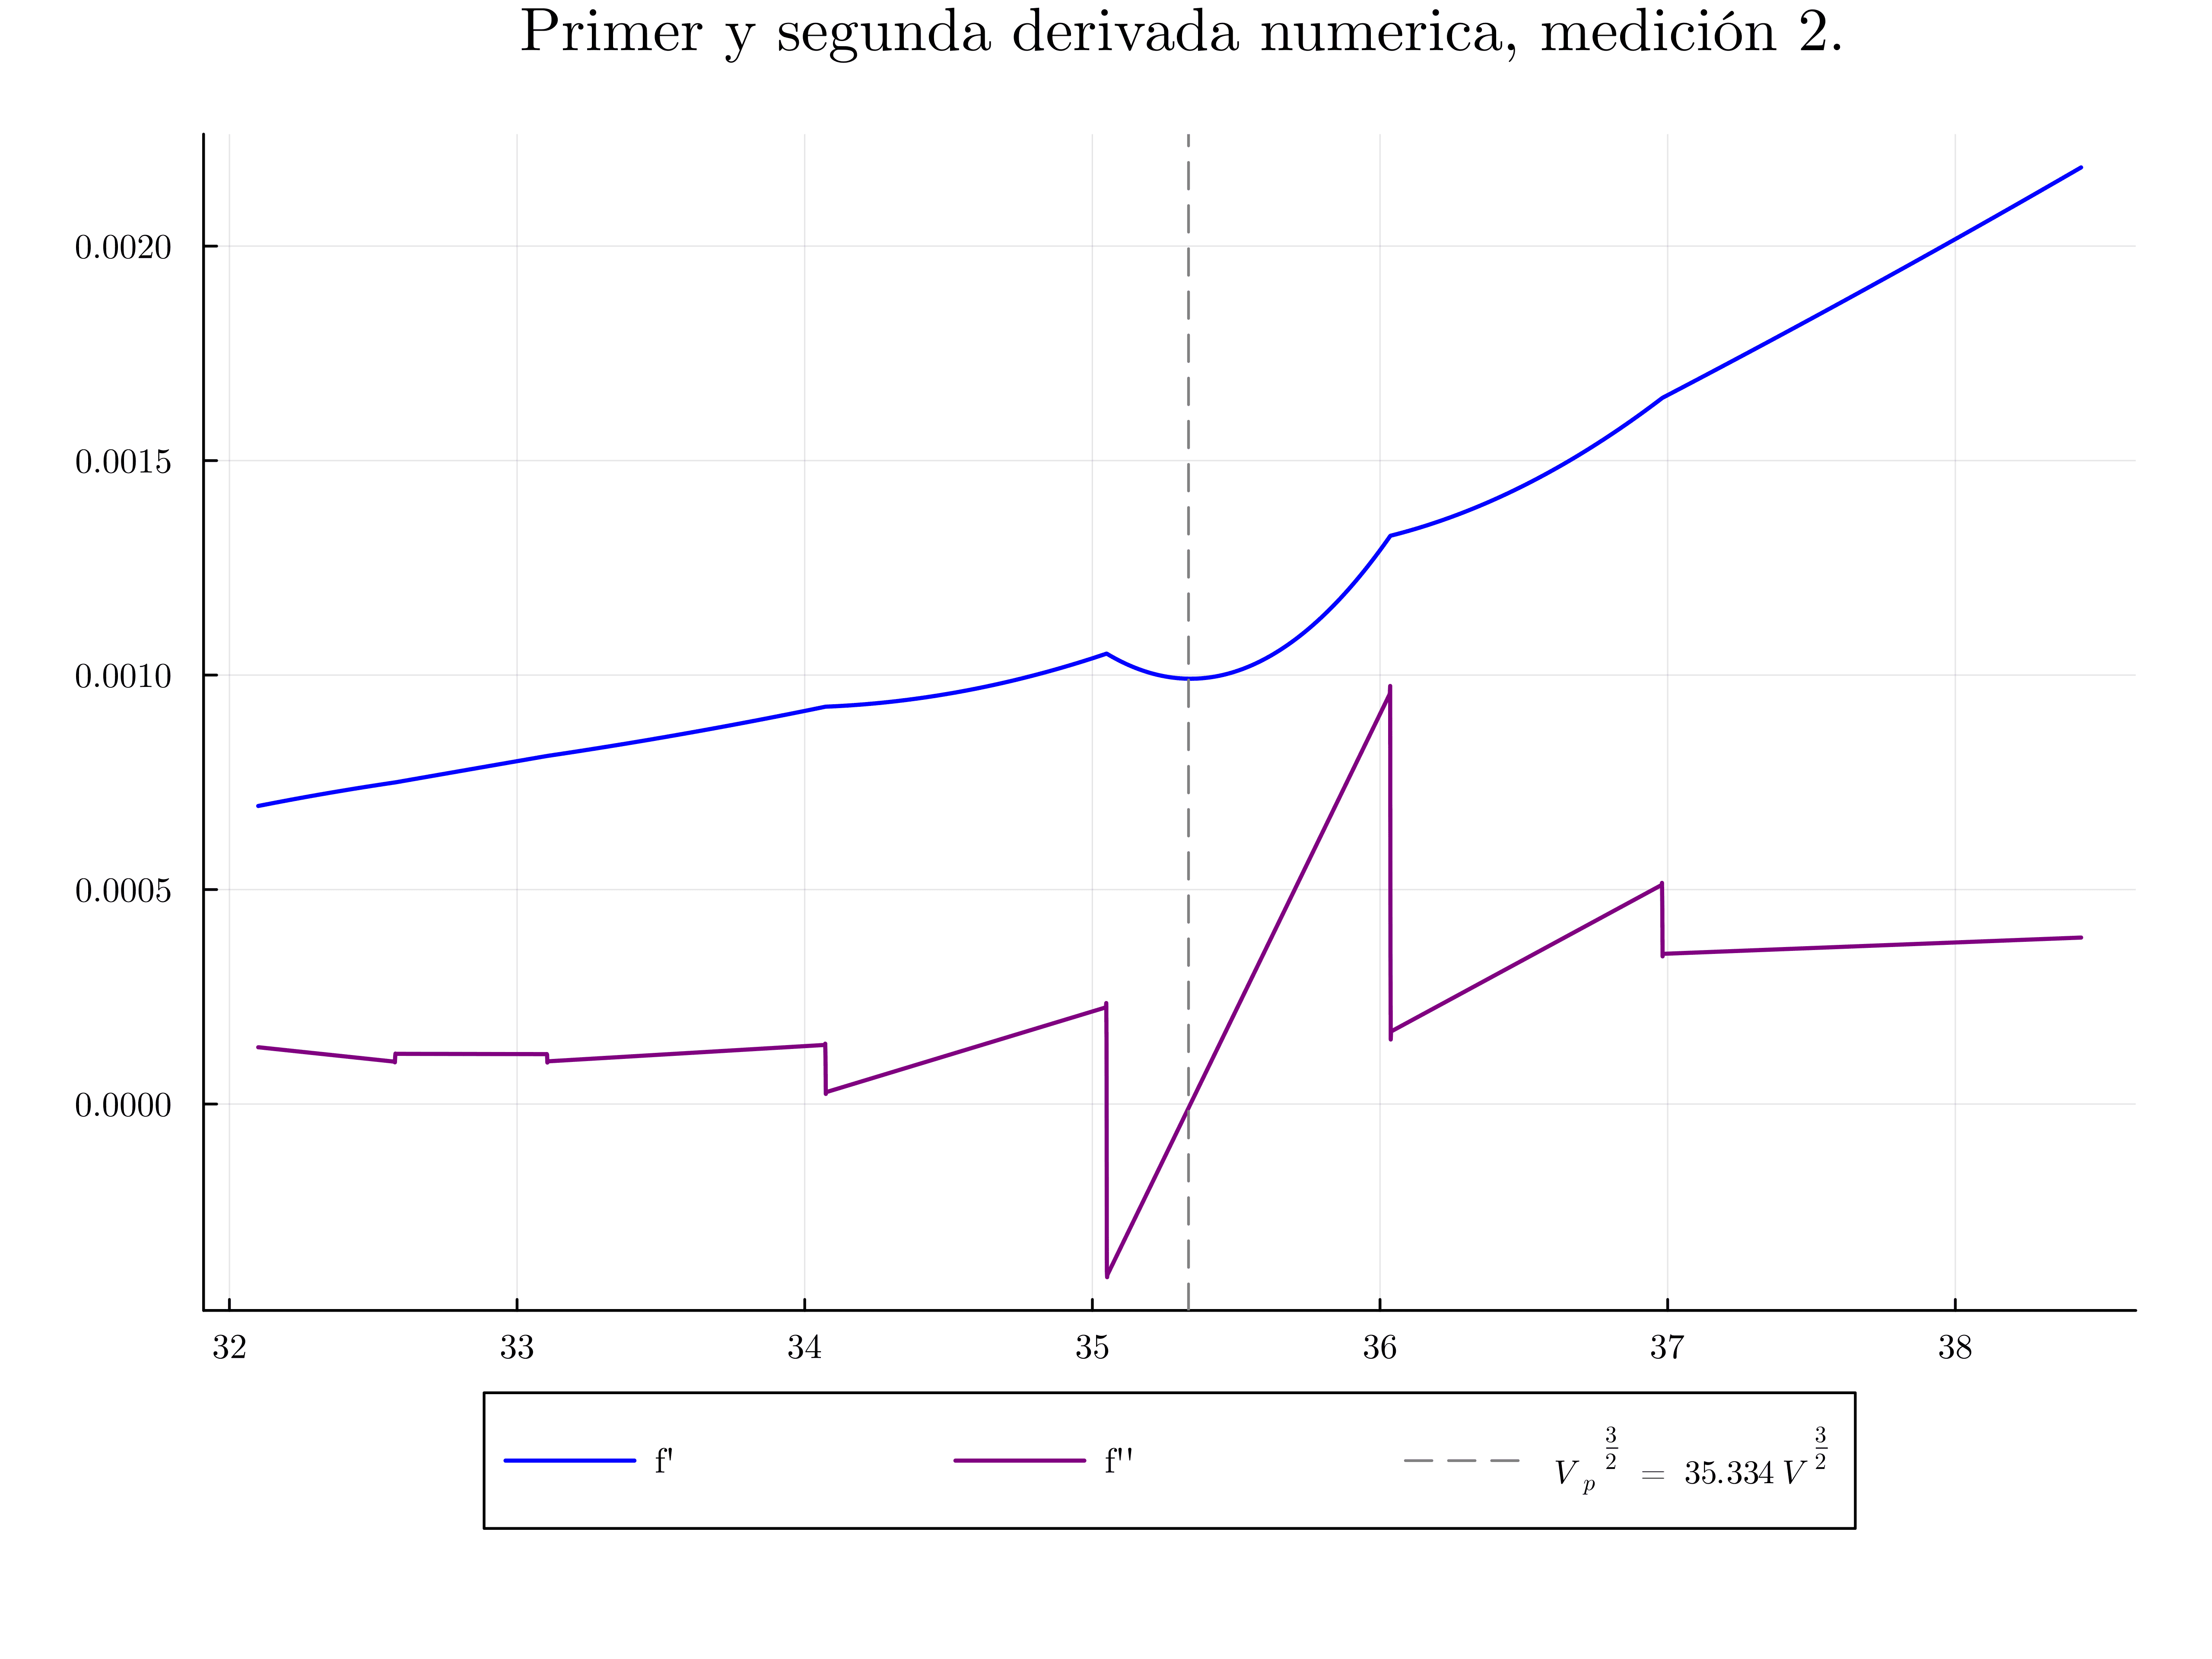
\includegraphics[width=\linewidth]{img/potderps2.png}
	\caption{Barrido n°: 2}
	\label{fig:potderps2}
\end{subfigure}

\end{figure}

% segundo bloque de figuras
\begin{figure}[H]
\ContinuedFloat
\centering
\begin{subfigure}[b]{0.49\textwidth}
	\centering
	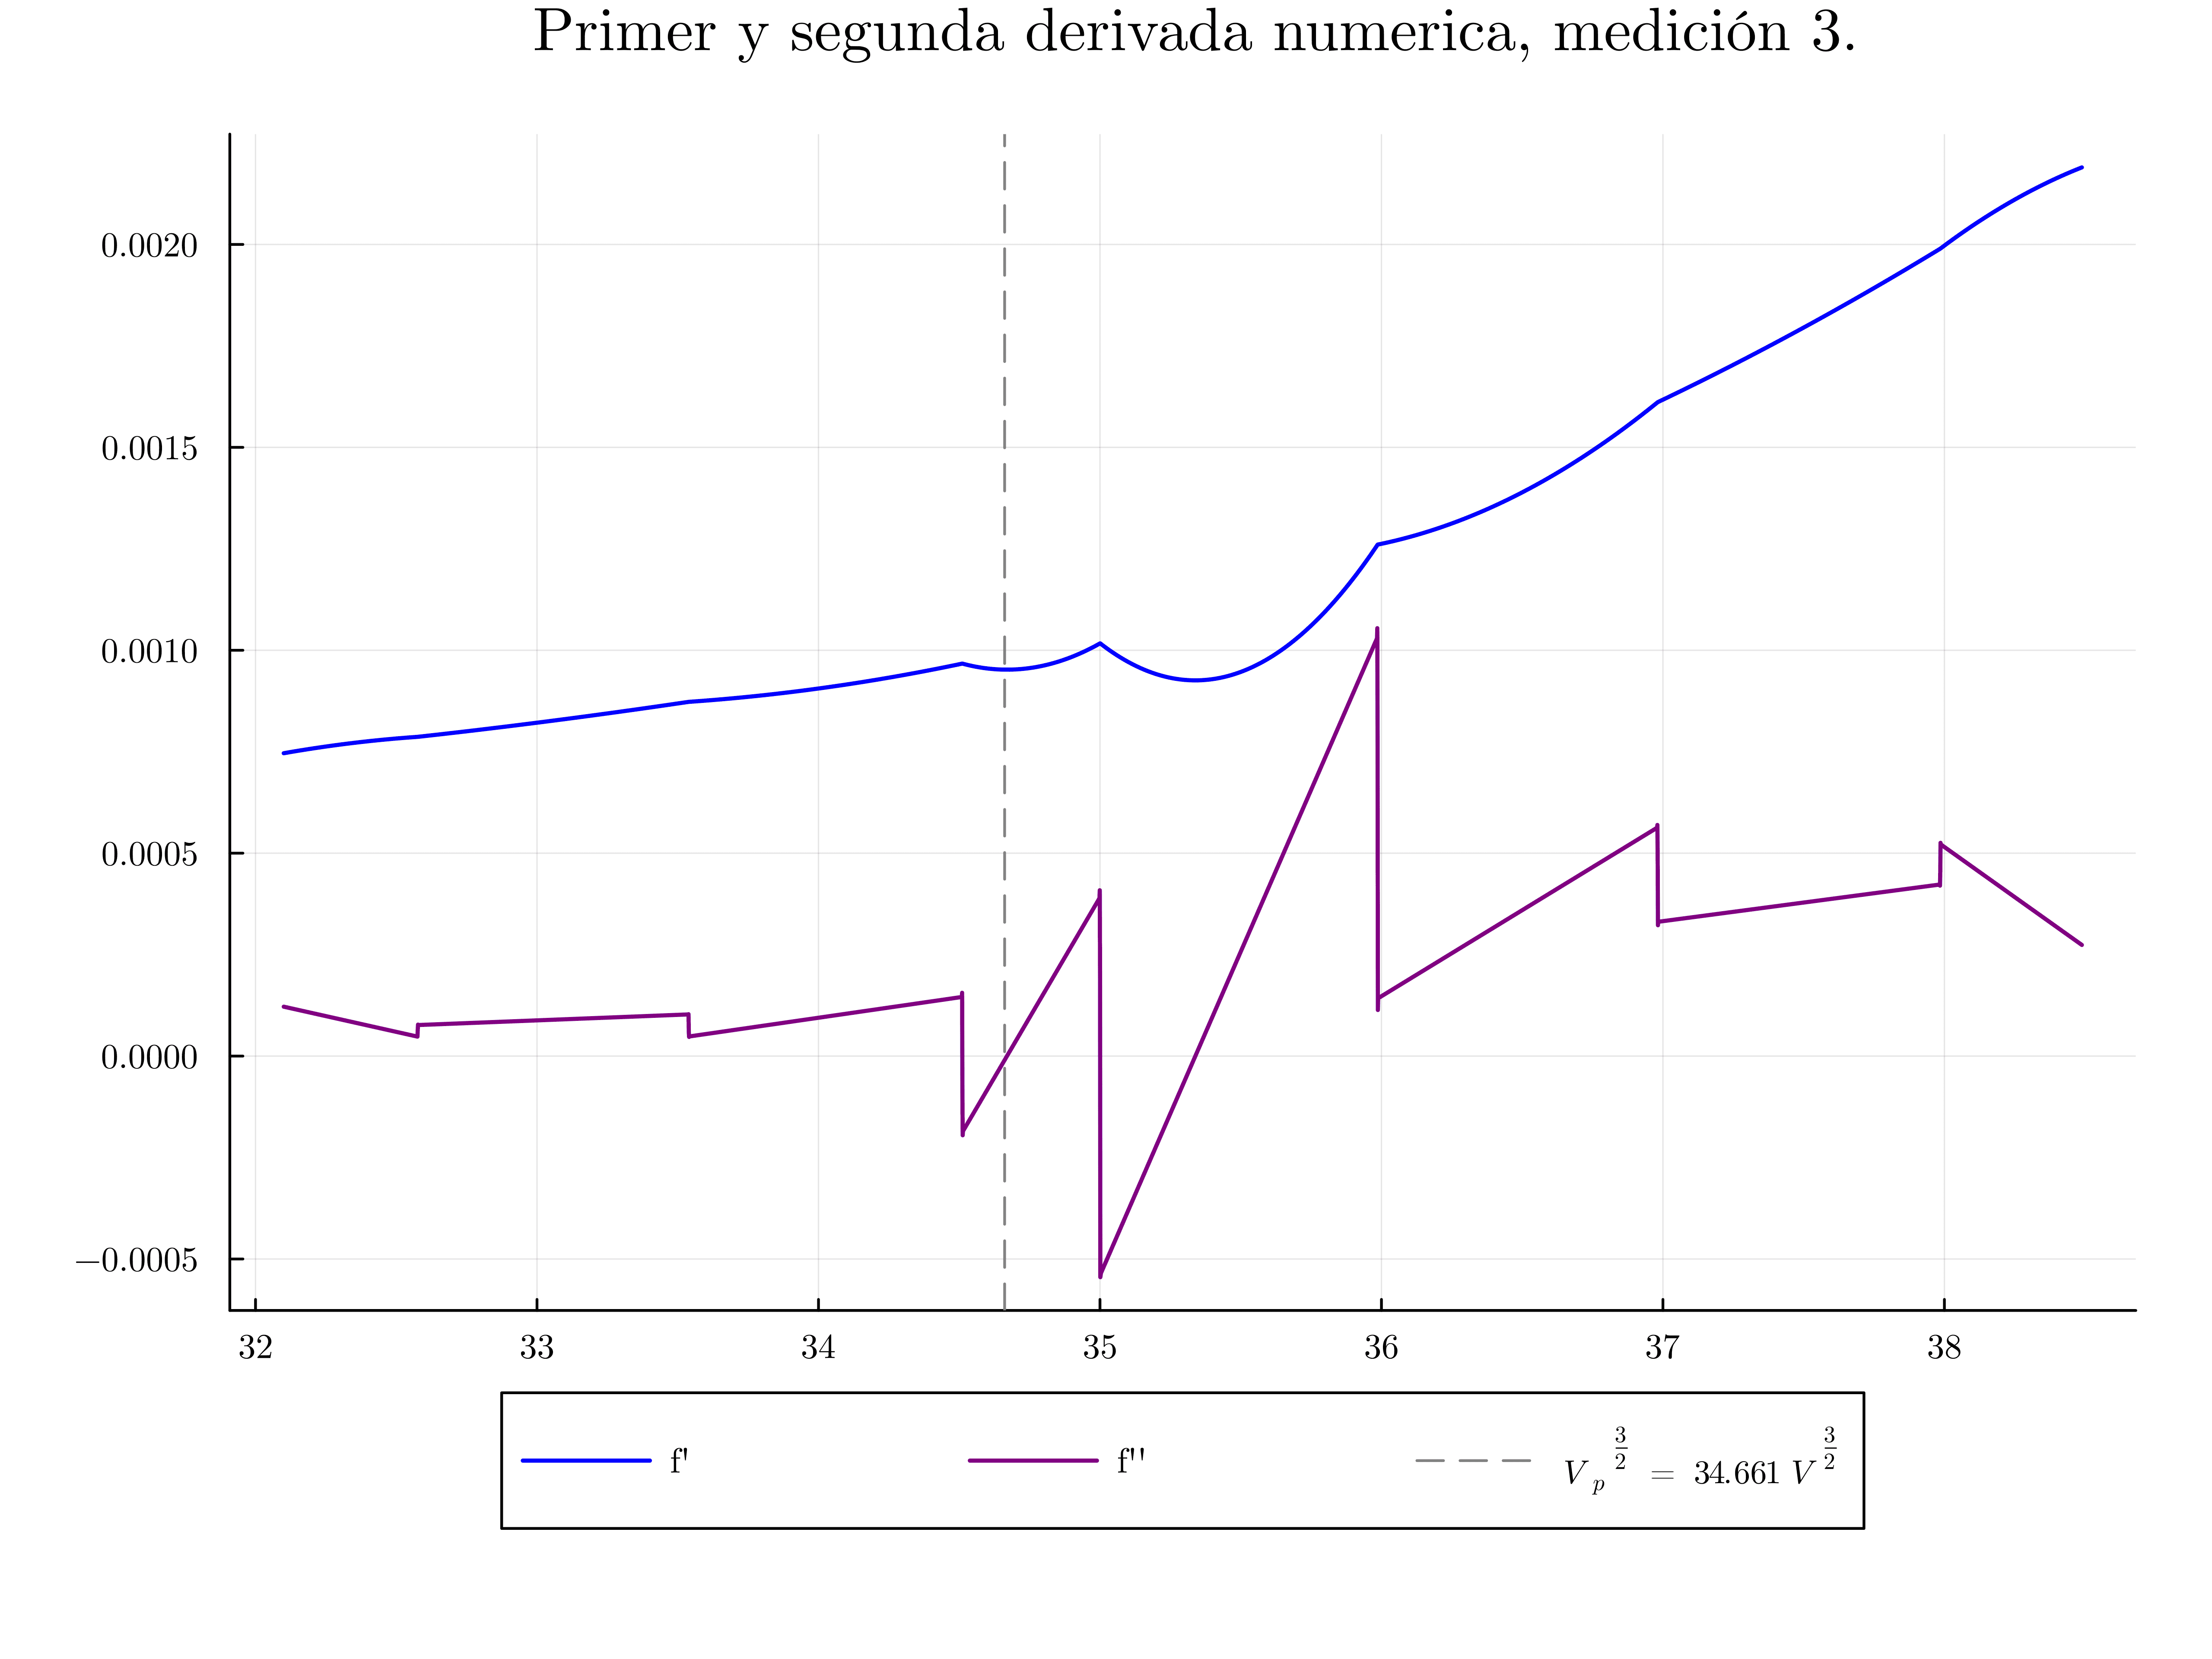
\includegraphics[width=\linewidth]{img/potderps3.png}
	\caption{Barrido n°: 3}
	\label{fig:potderps3}
\end{subfigure}
\hfill
\begin{subfigure}[b]{0.49\textwidth}
	\centering
	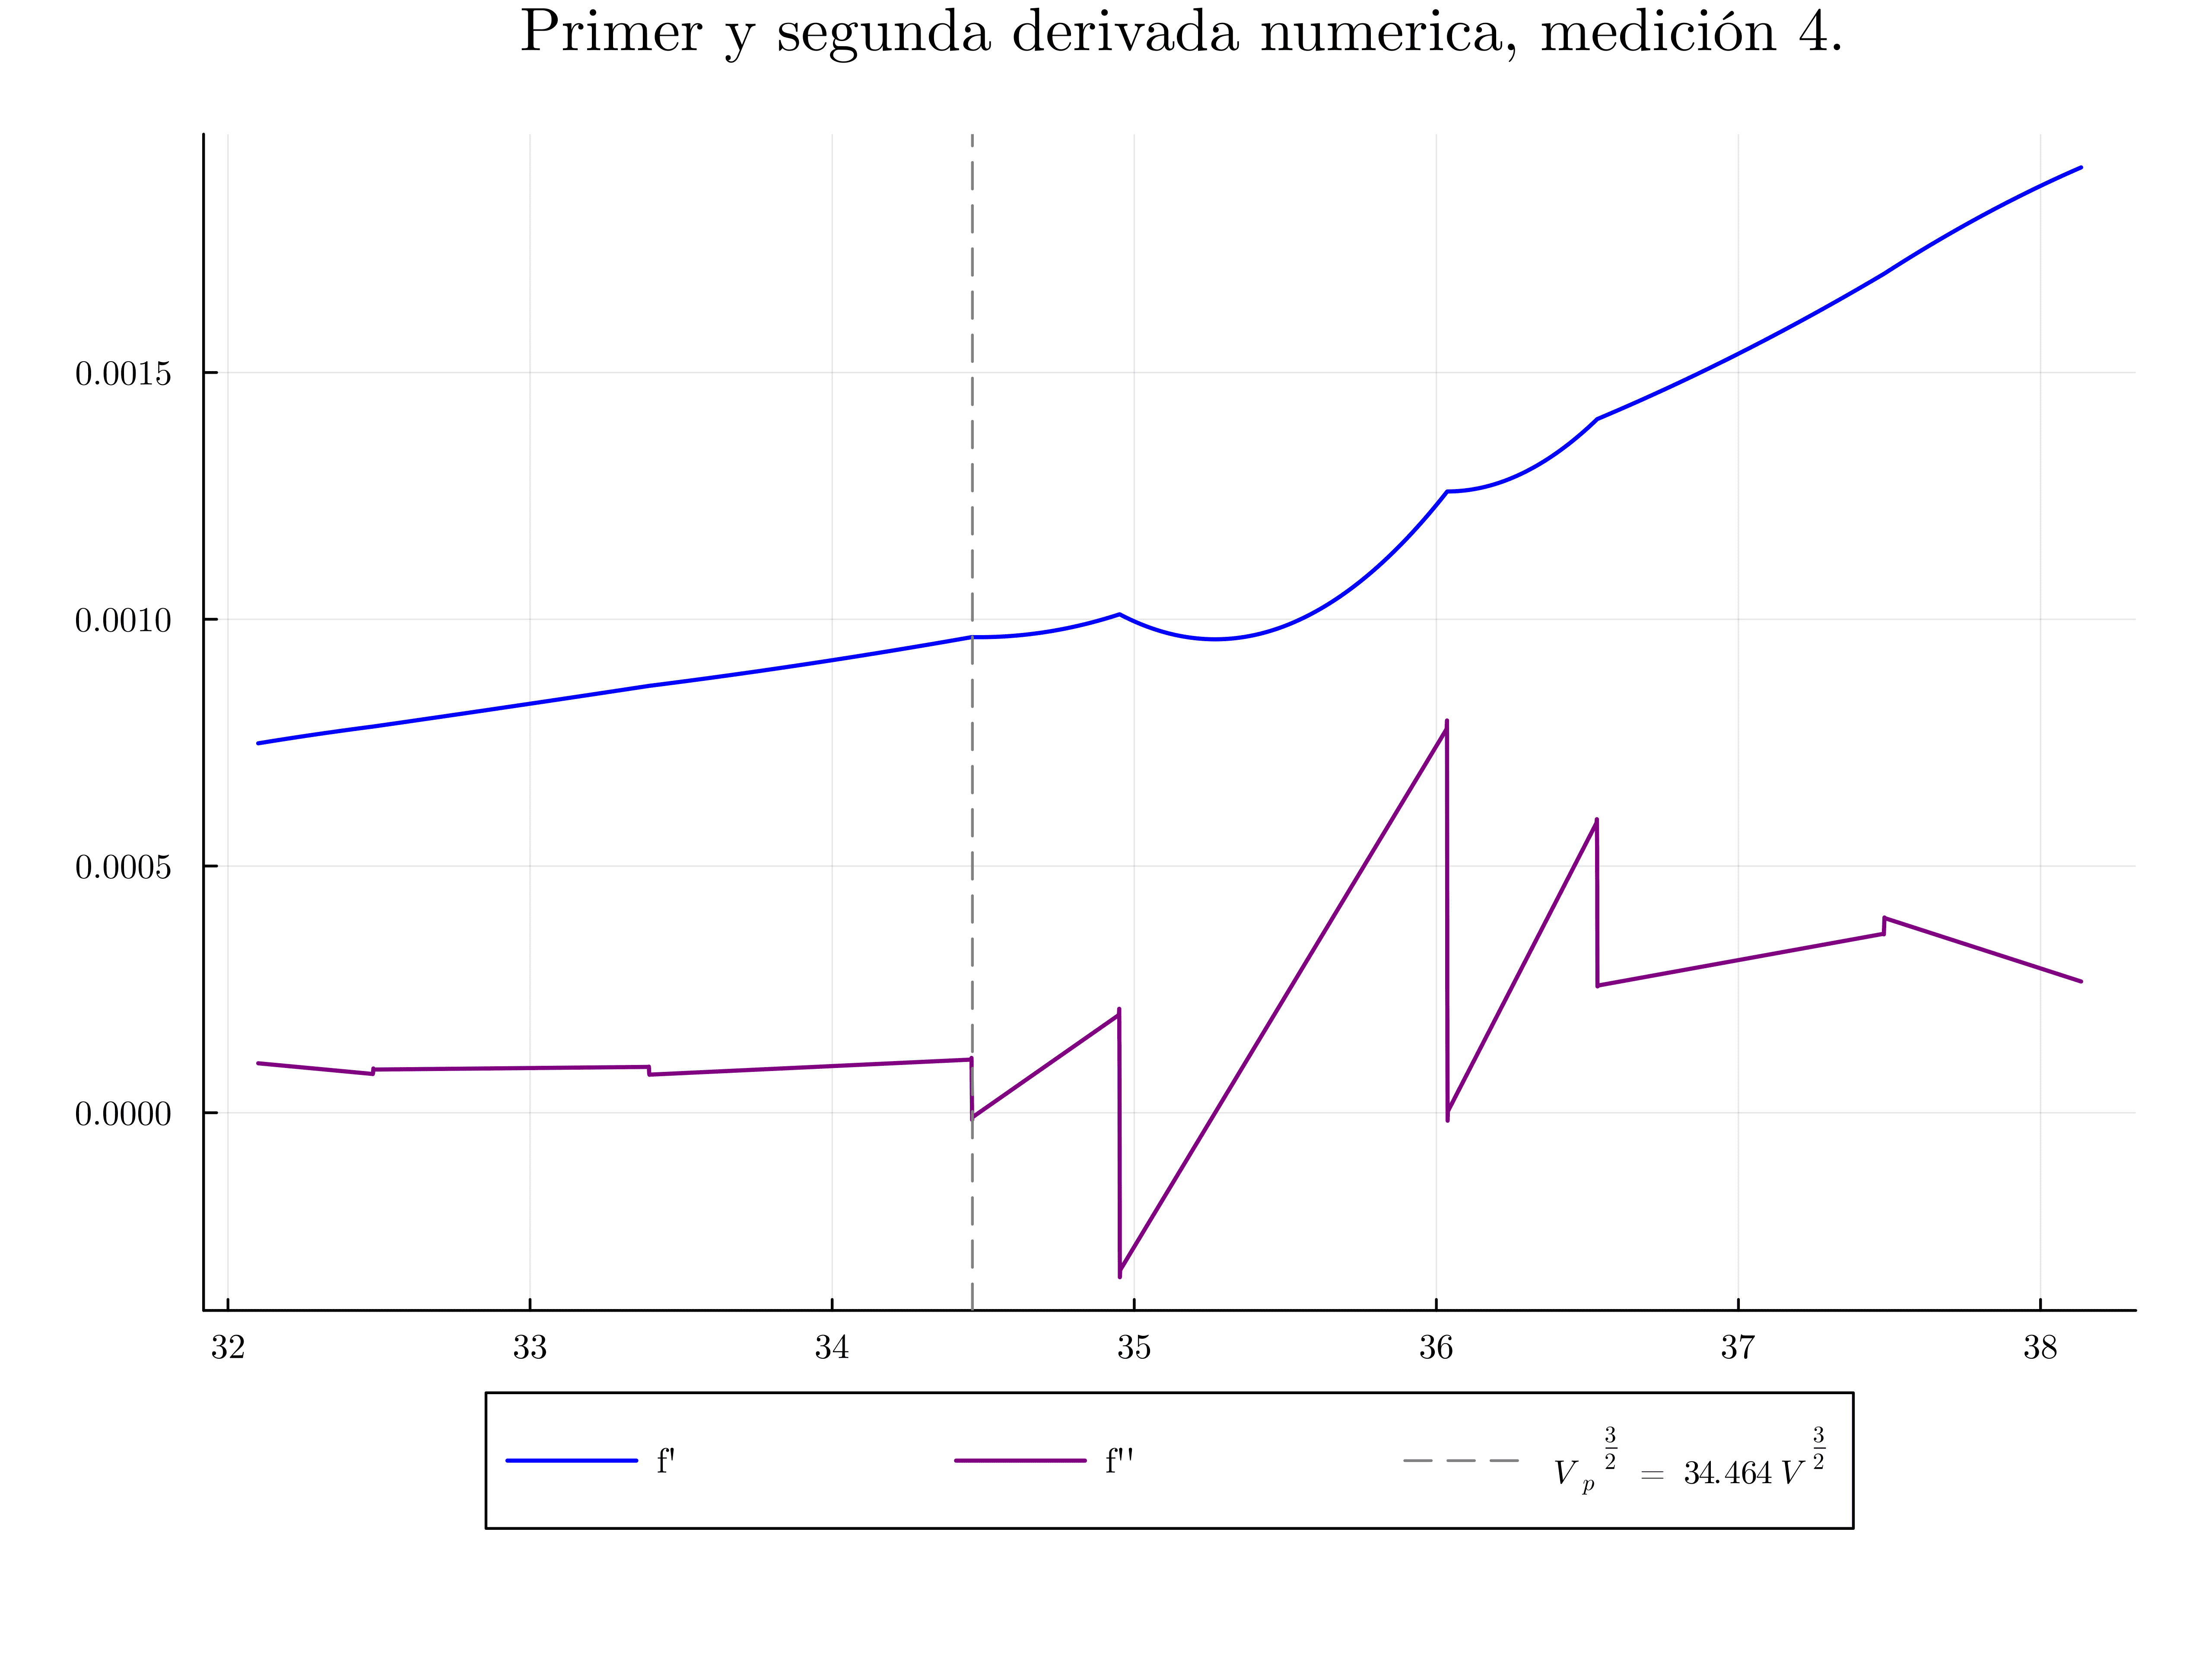
\includegraphics[width=\linewidth]{img/potderps4.png}
	\caption{Barrido n°: 4}
	\label{fig:potderps4}
\end{subfigure}

\end{figure}

% teercer bloque de figuras
\begin{figure}[H]
\ContinuedFloat % Indica que esta figura continúa de la anterior
\centering
\begin{subfigure}[b]{0.49\textwidth}
	\centering
	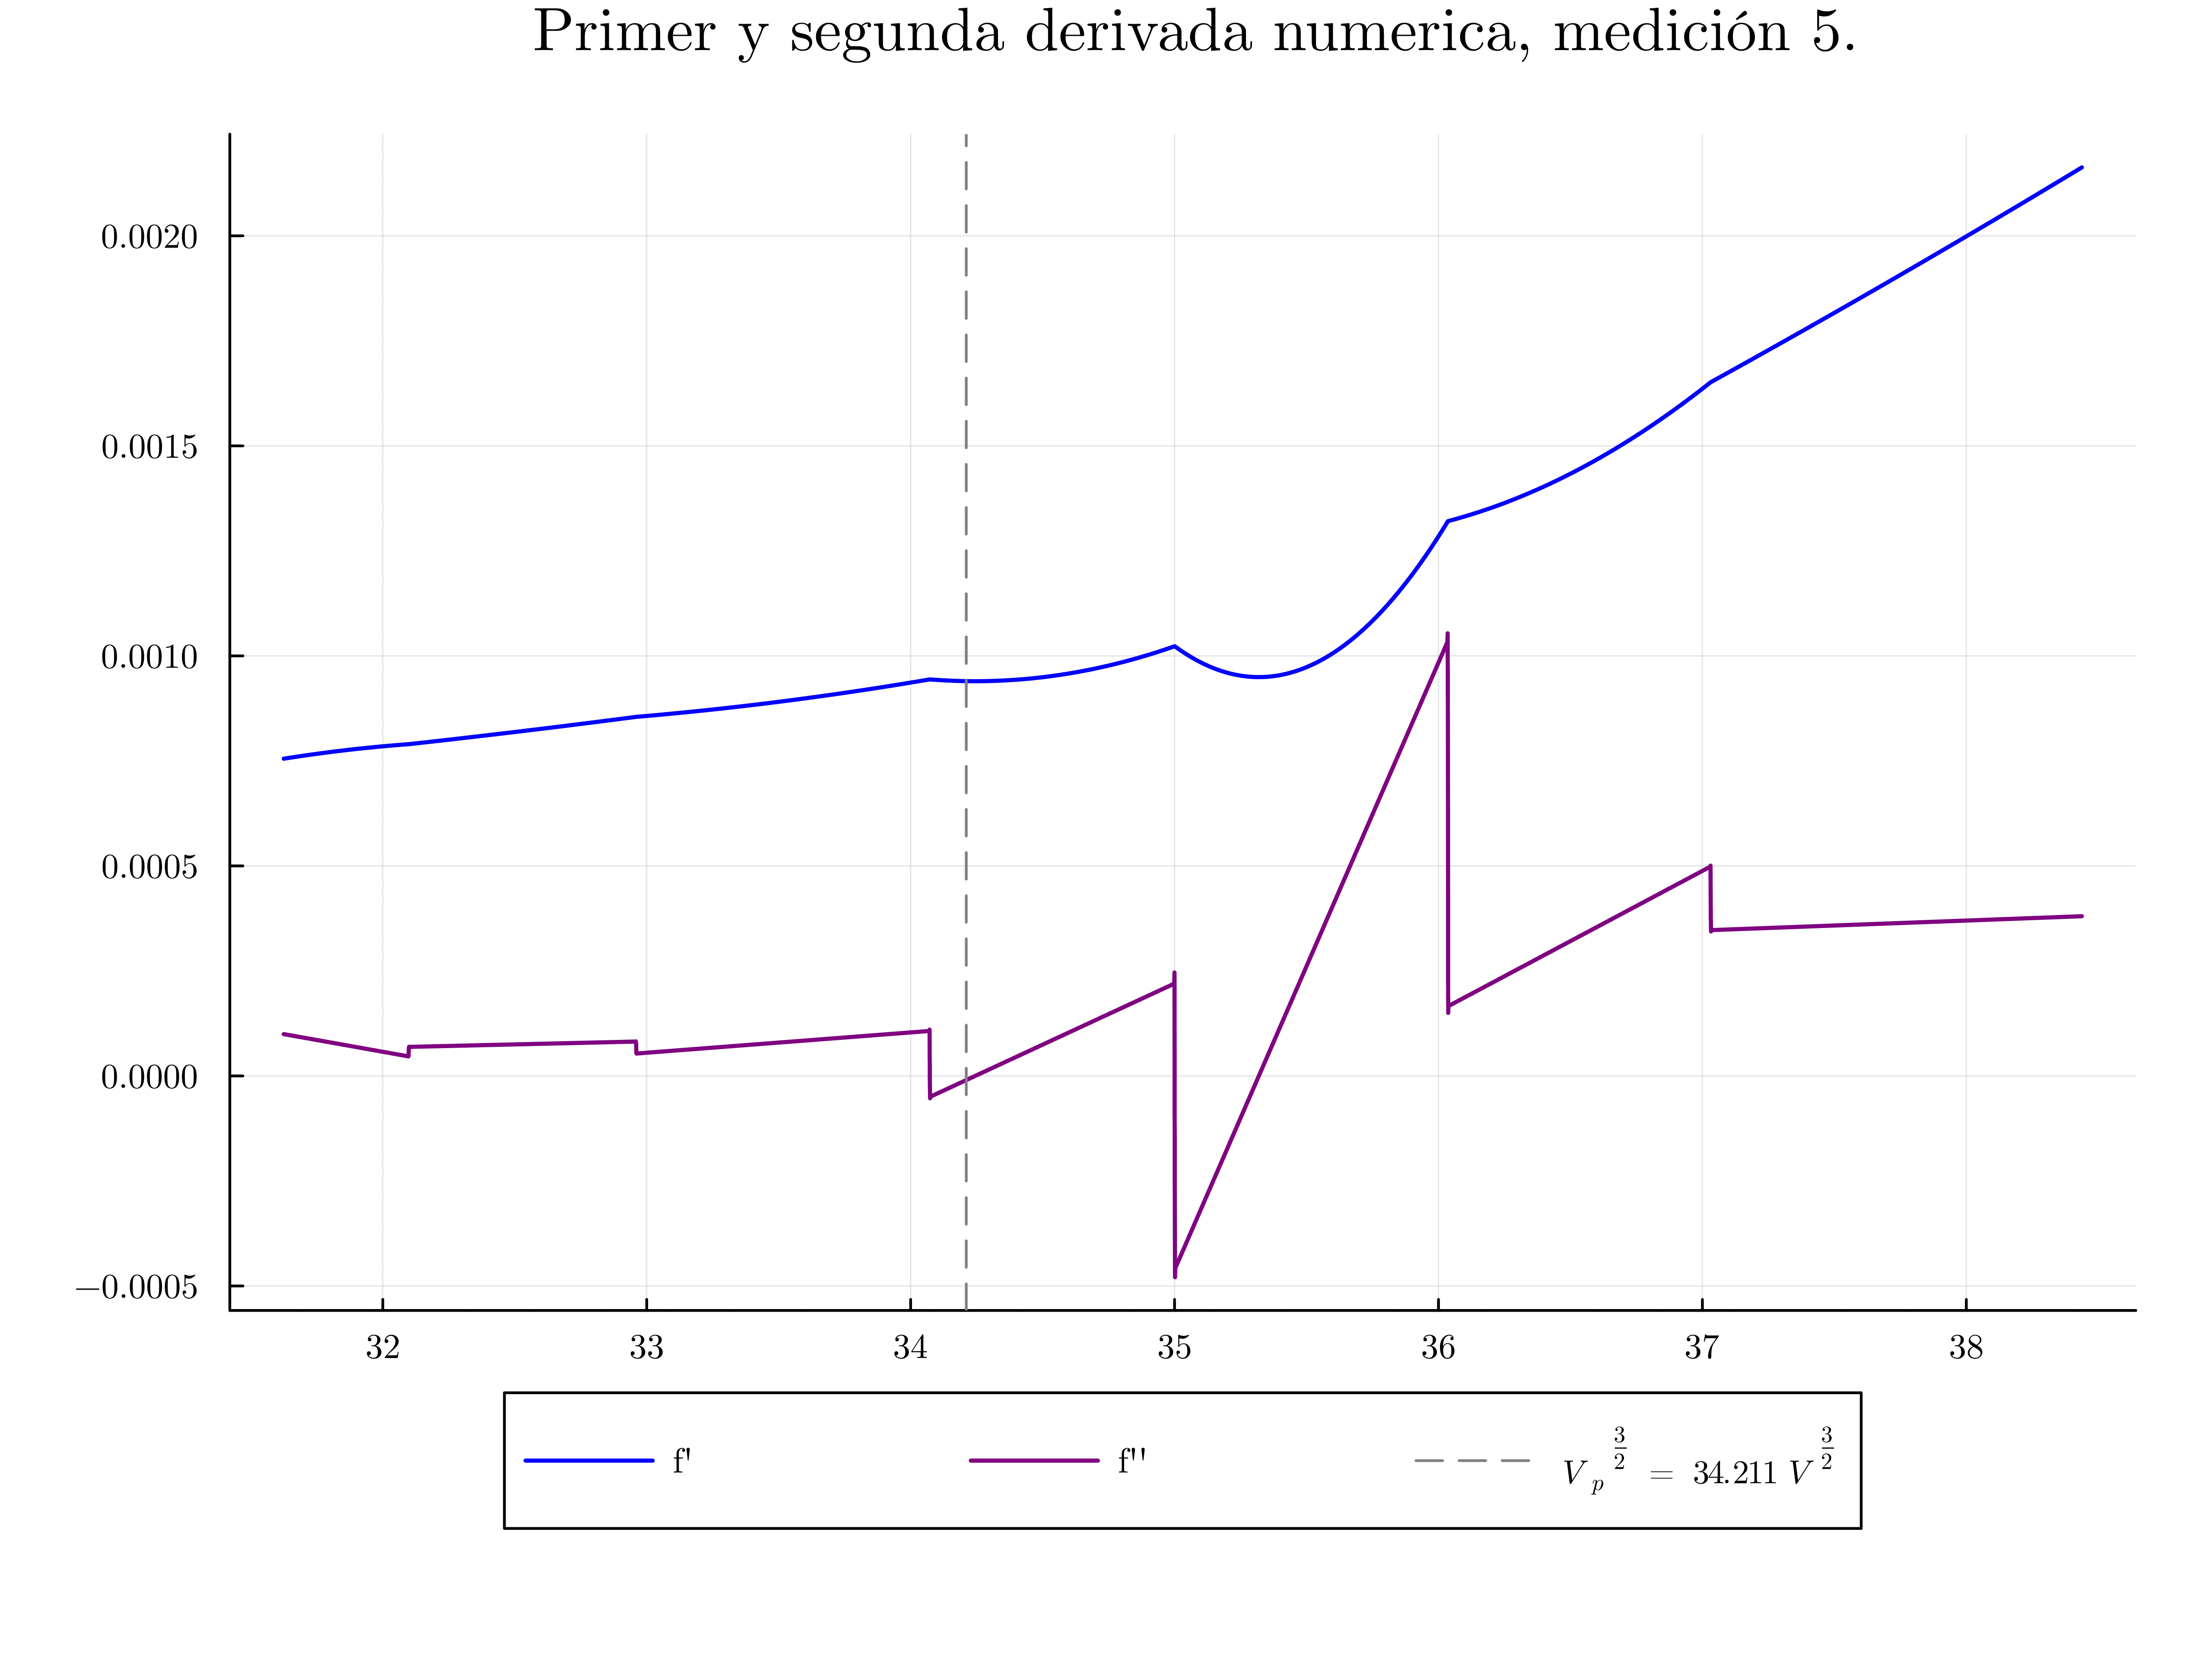
\includegraphics[width=\linewidth]{img/potderps5.png}
	\caption{Barrido n°: 5}
	\label{fig:potderps5}
\end{subfigure}
\hfill
\begin{subfigure}[b]{0.49\textwidth}
	\centering
	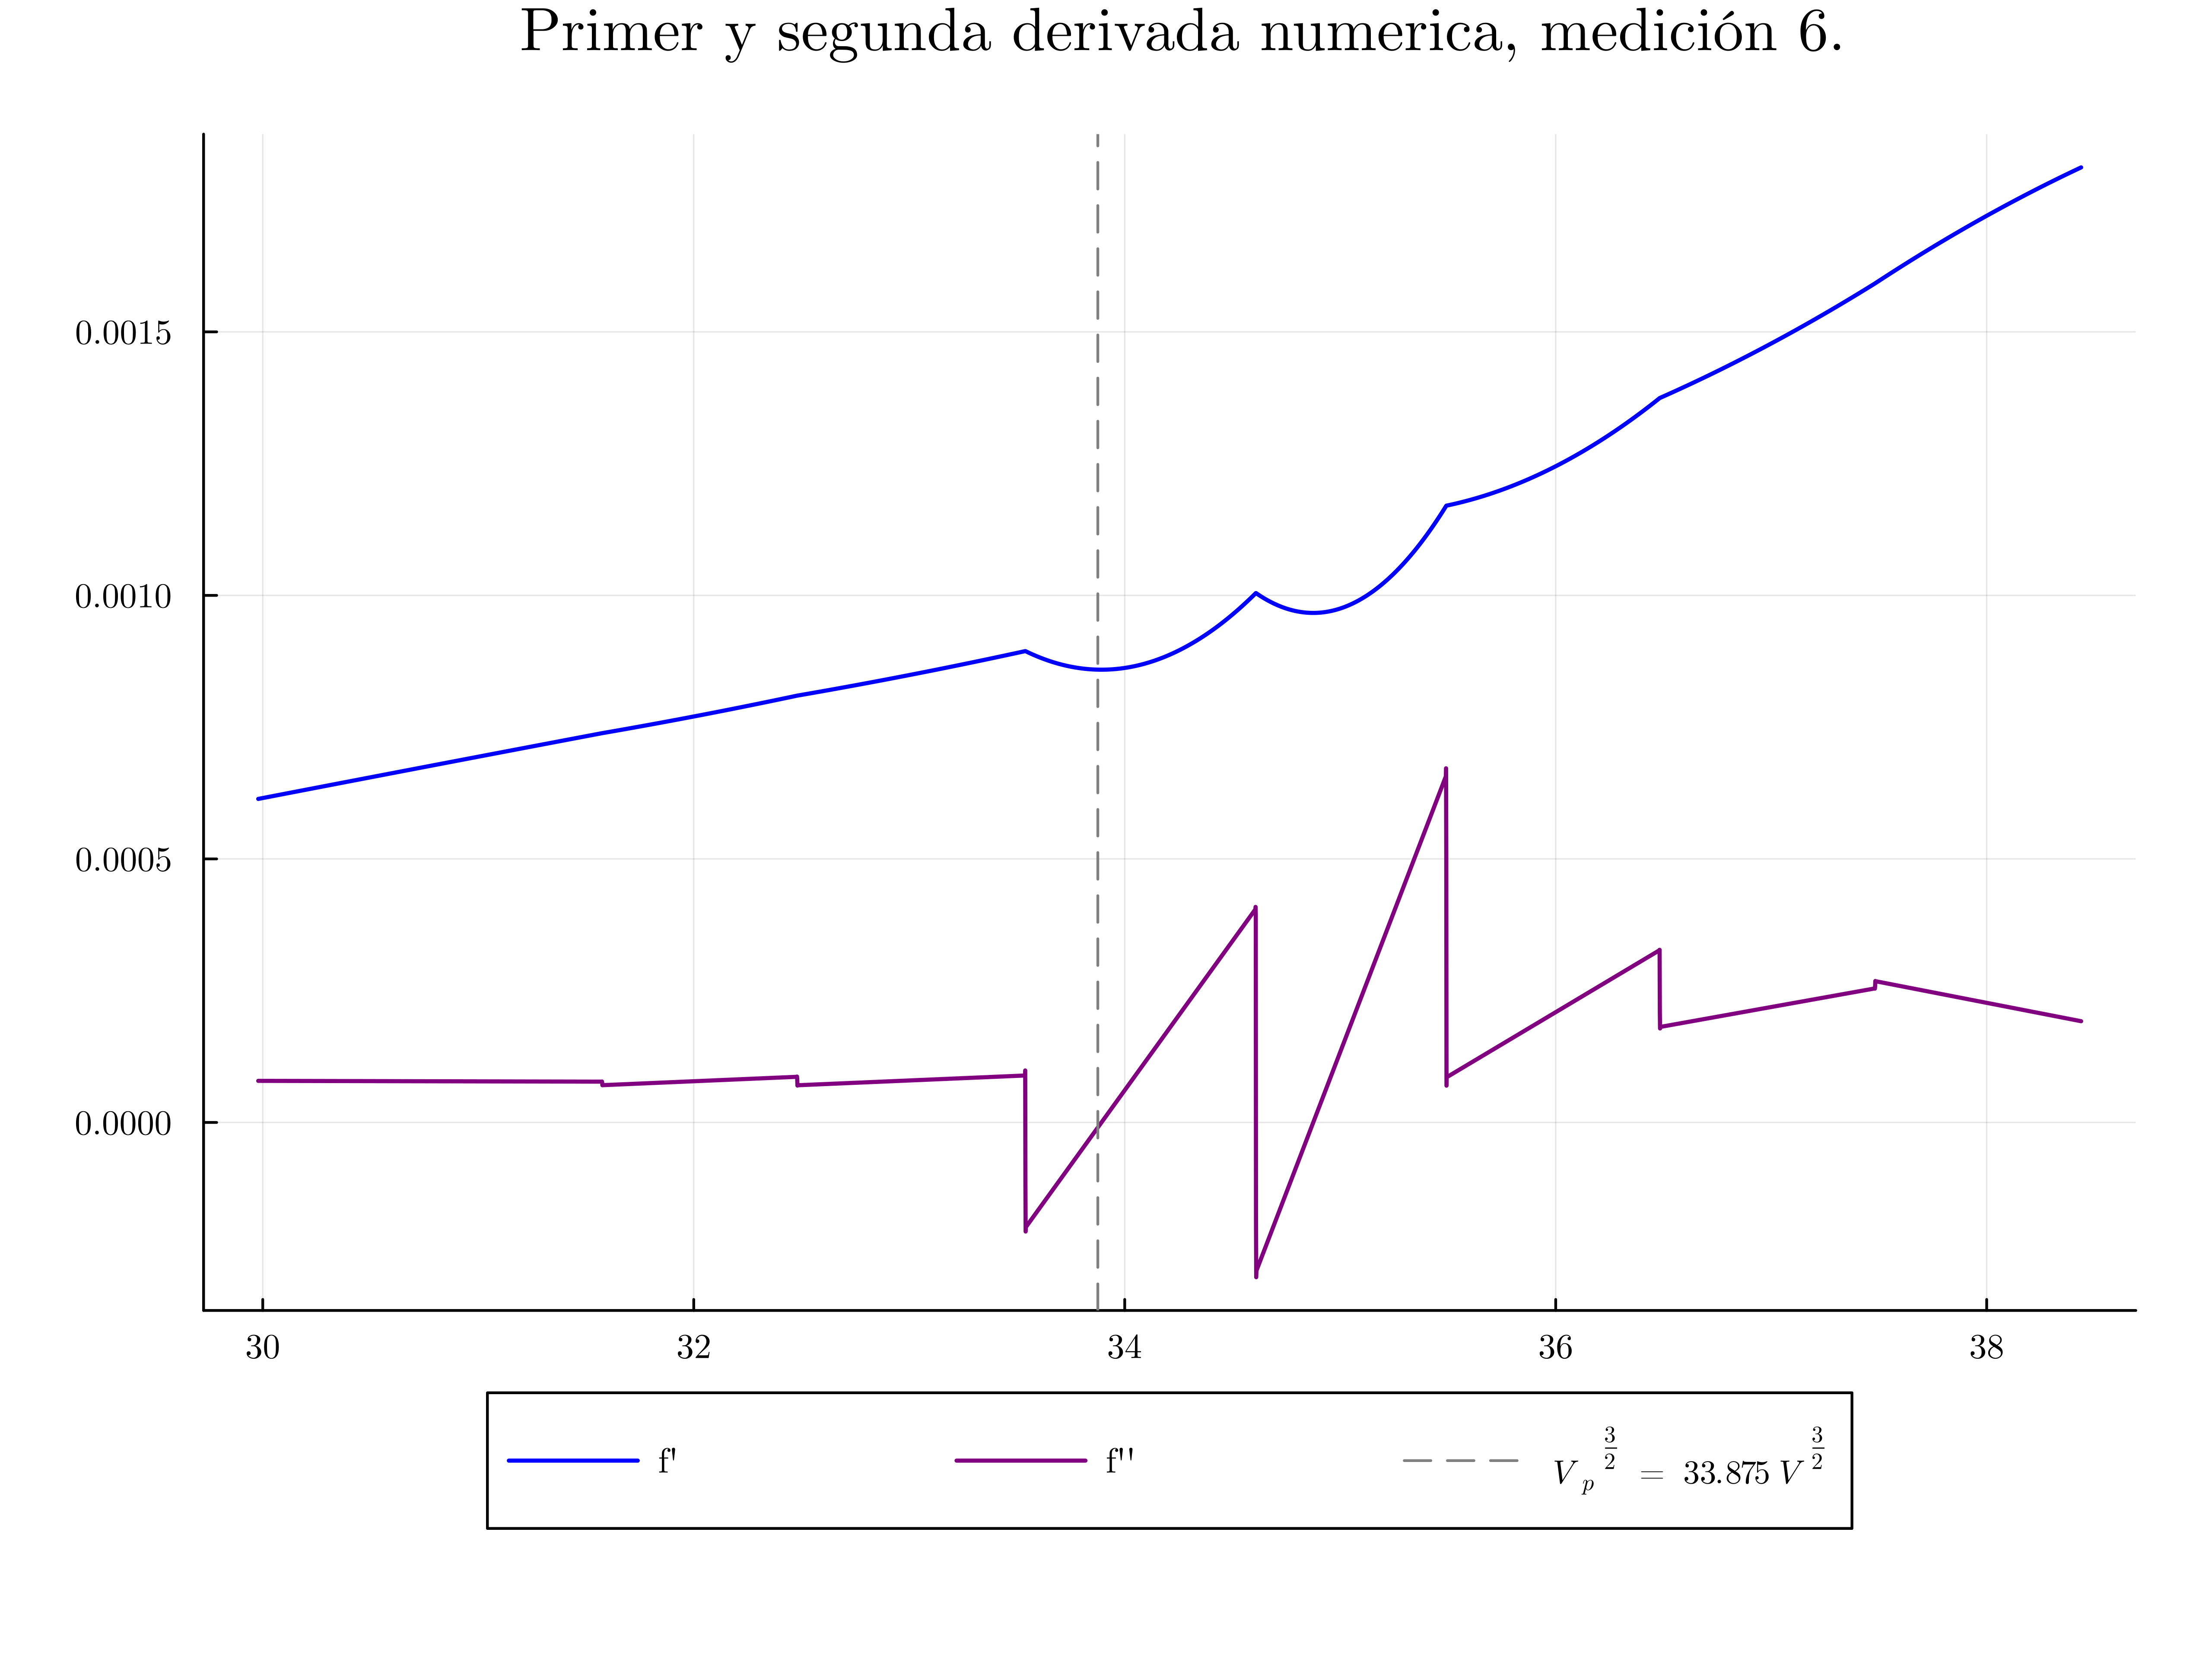
\includegraphics[width=\linewidth]{img/potderps6.png}
	\caption{Barrido n°: 6}
	\label{fig:potderps6}
\end{subfigure}

\end{figure}

% cuarto bloque de figuras
\begin{figure}[H]
\ContinuedFloat % Indica que esta figura continúa de la anterior
\centering
\begin{subfigure}[b]{0.49\textwidth}
	\centering
	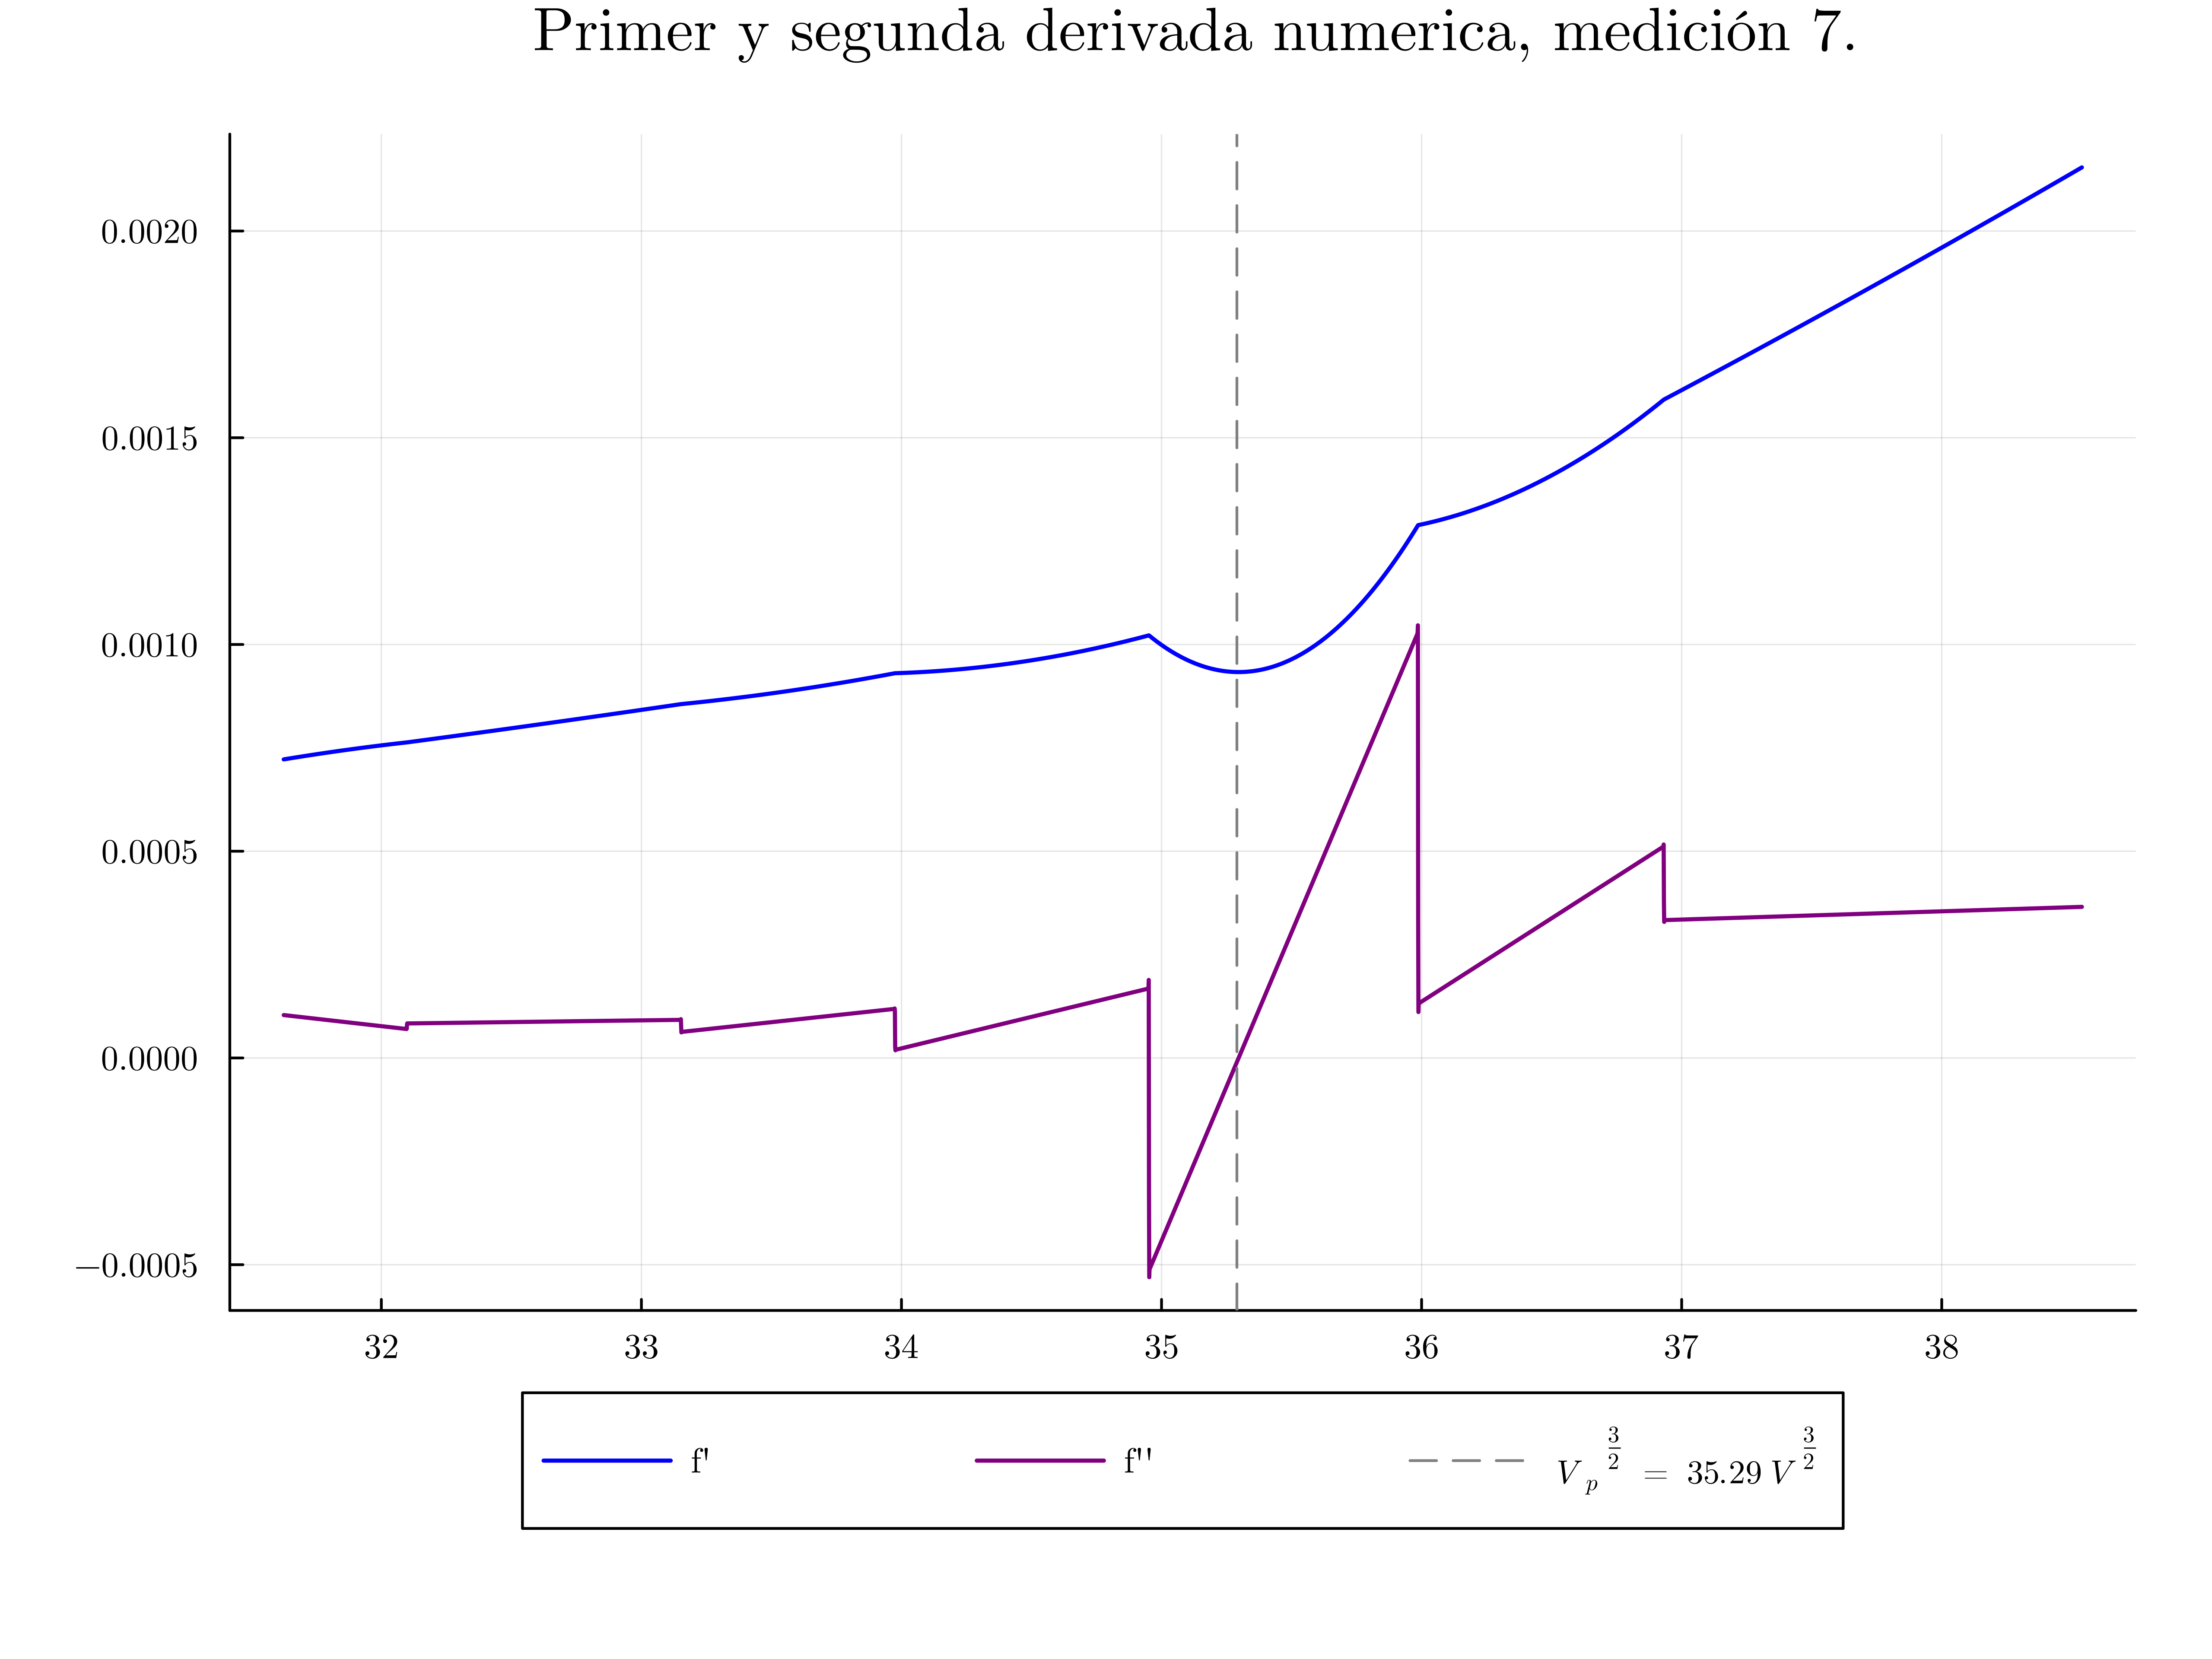
\includegraphics[width=\linewidth]{img/potderps7.png}
	\caption{Barrido n°: 7}
	\label{fig:potderps7}
\end{subfigure}
\hfill
\begin{subfigure}[b]{0.49\textwidth}
	\centering
	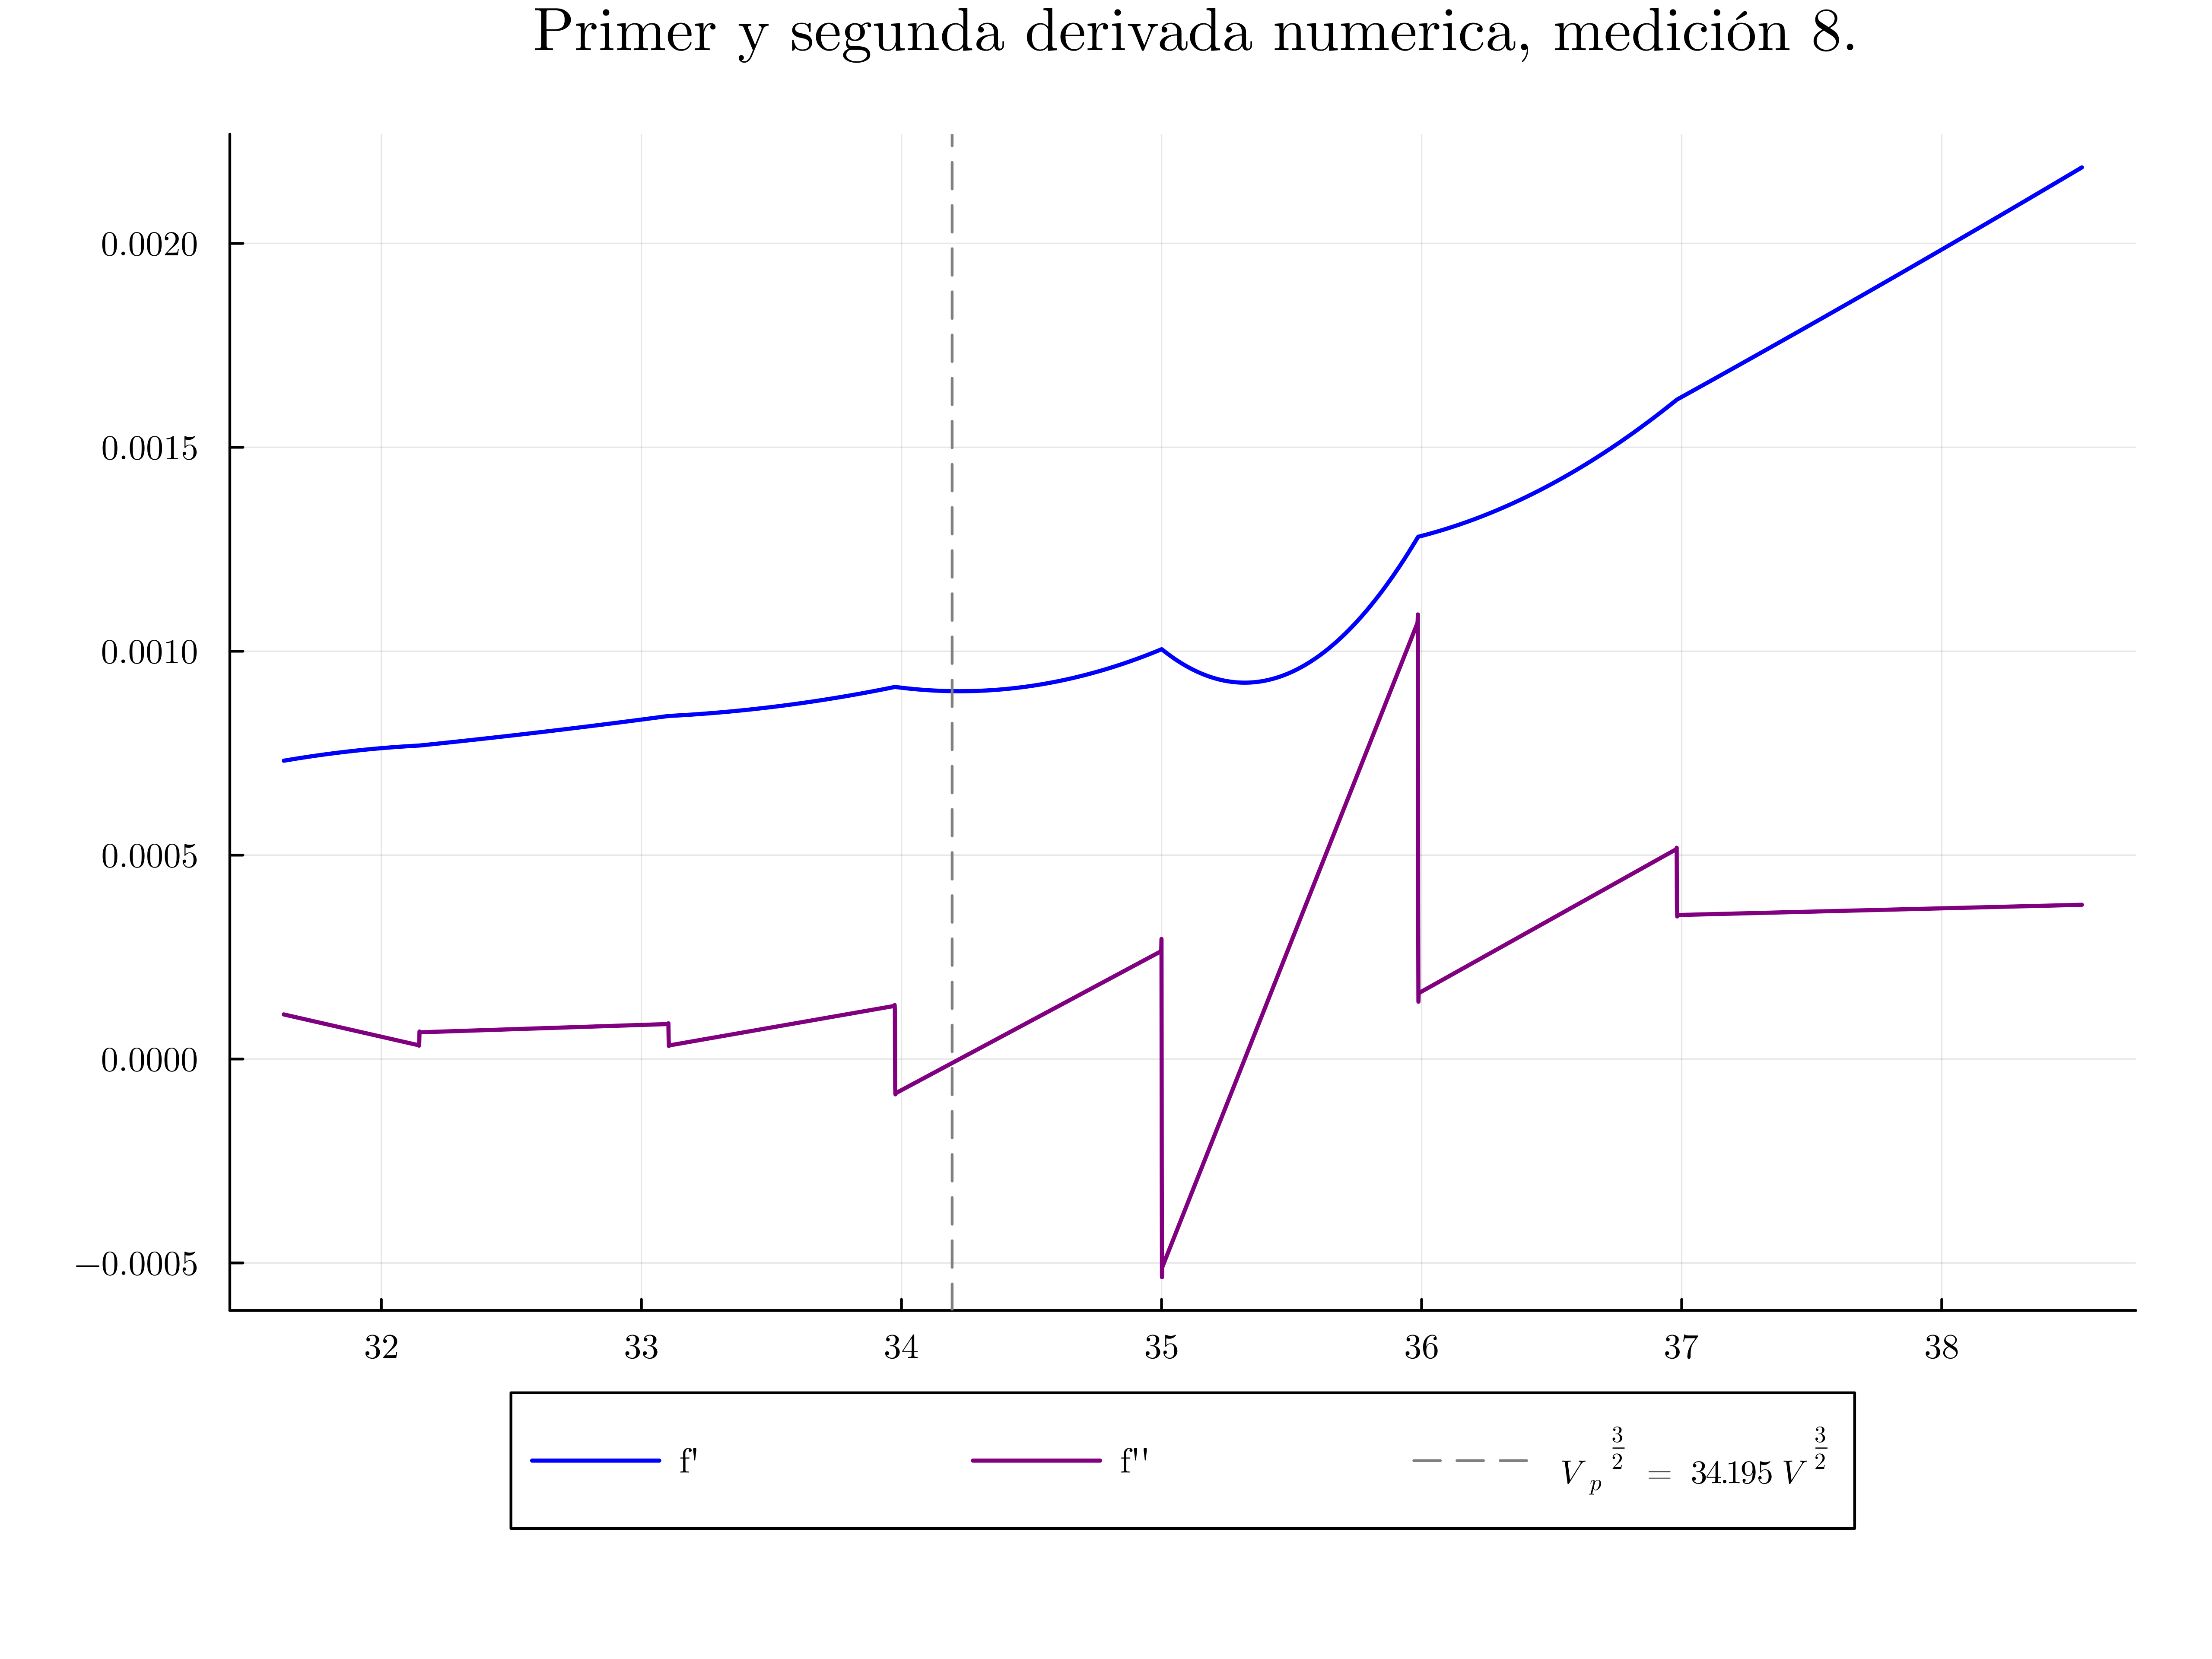
\includegraphics[width=\linewidth]{img/potderps8.png}
	\caption{Barrido n°: 8}
	\label{fig:potderps8}
\end{subfigure}
\end{figure}


% Últimas figuras
\begin{figure}[H]
\ContinuedFloat % Sigue con la misma numeración y caption
\centering
\begin{subfigure}[b]{0.49\textwidth}
	\centering
	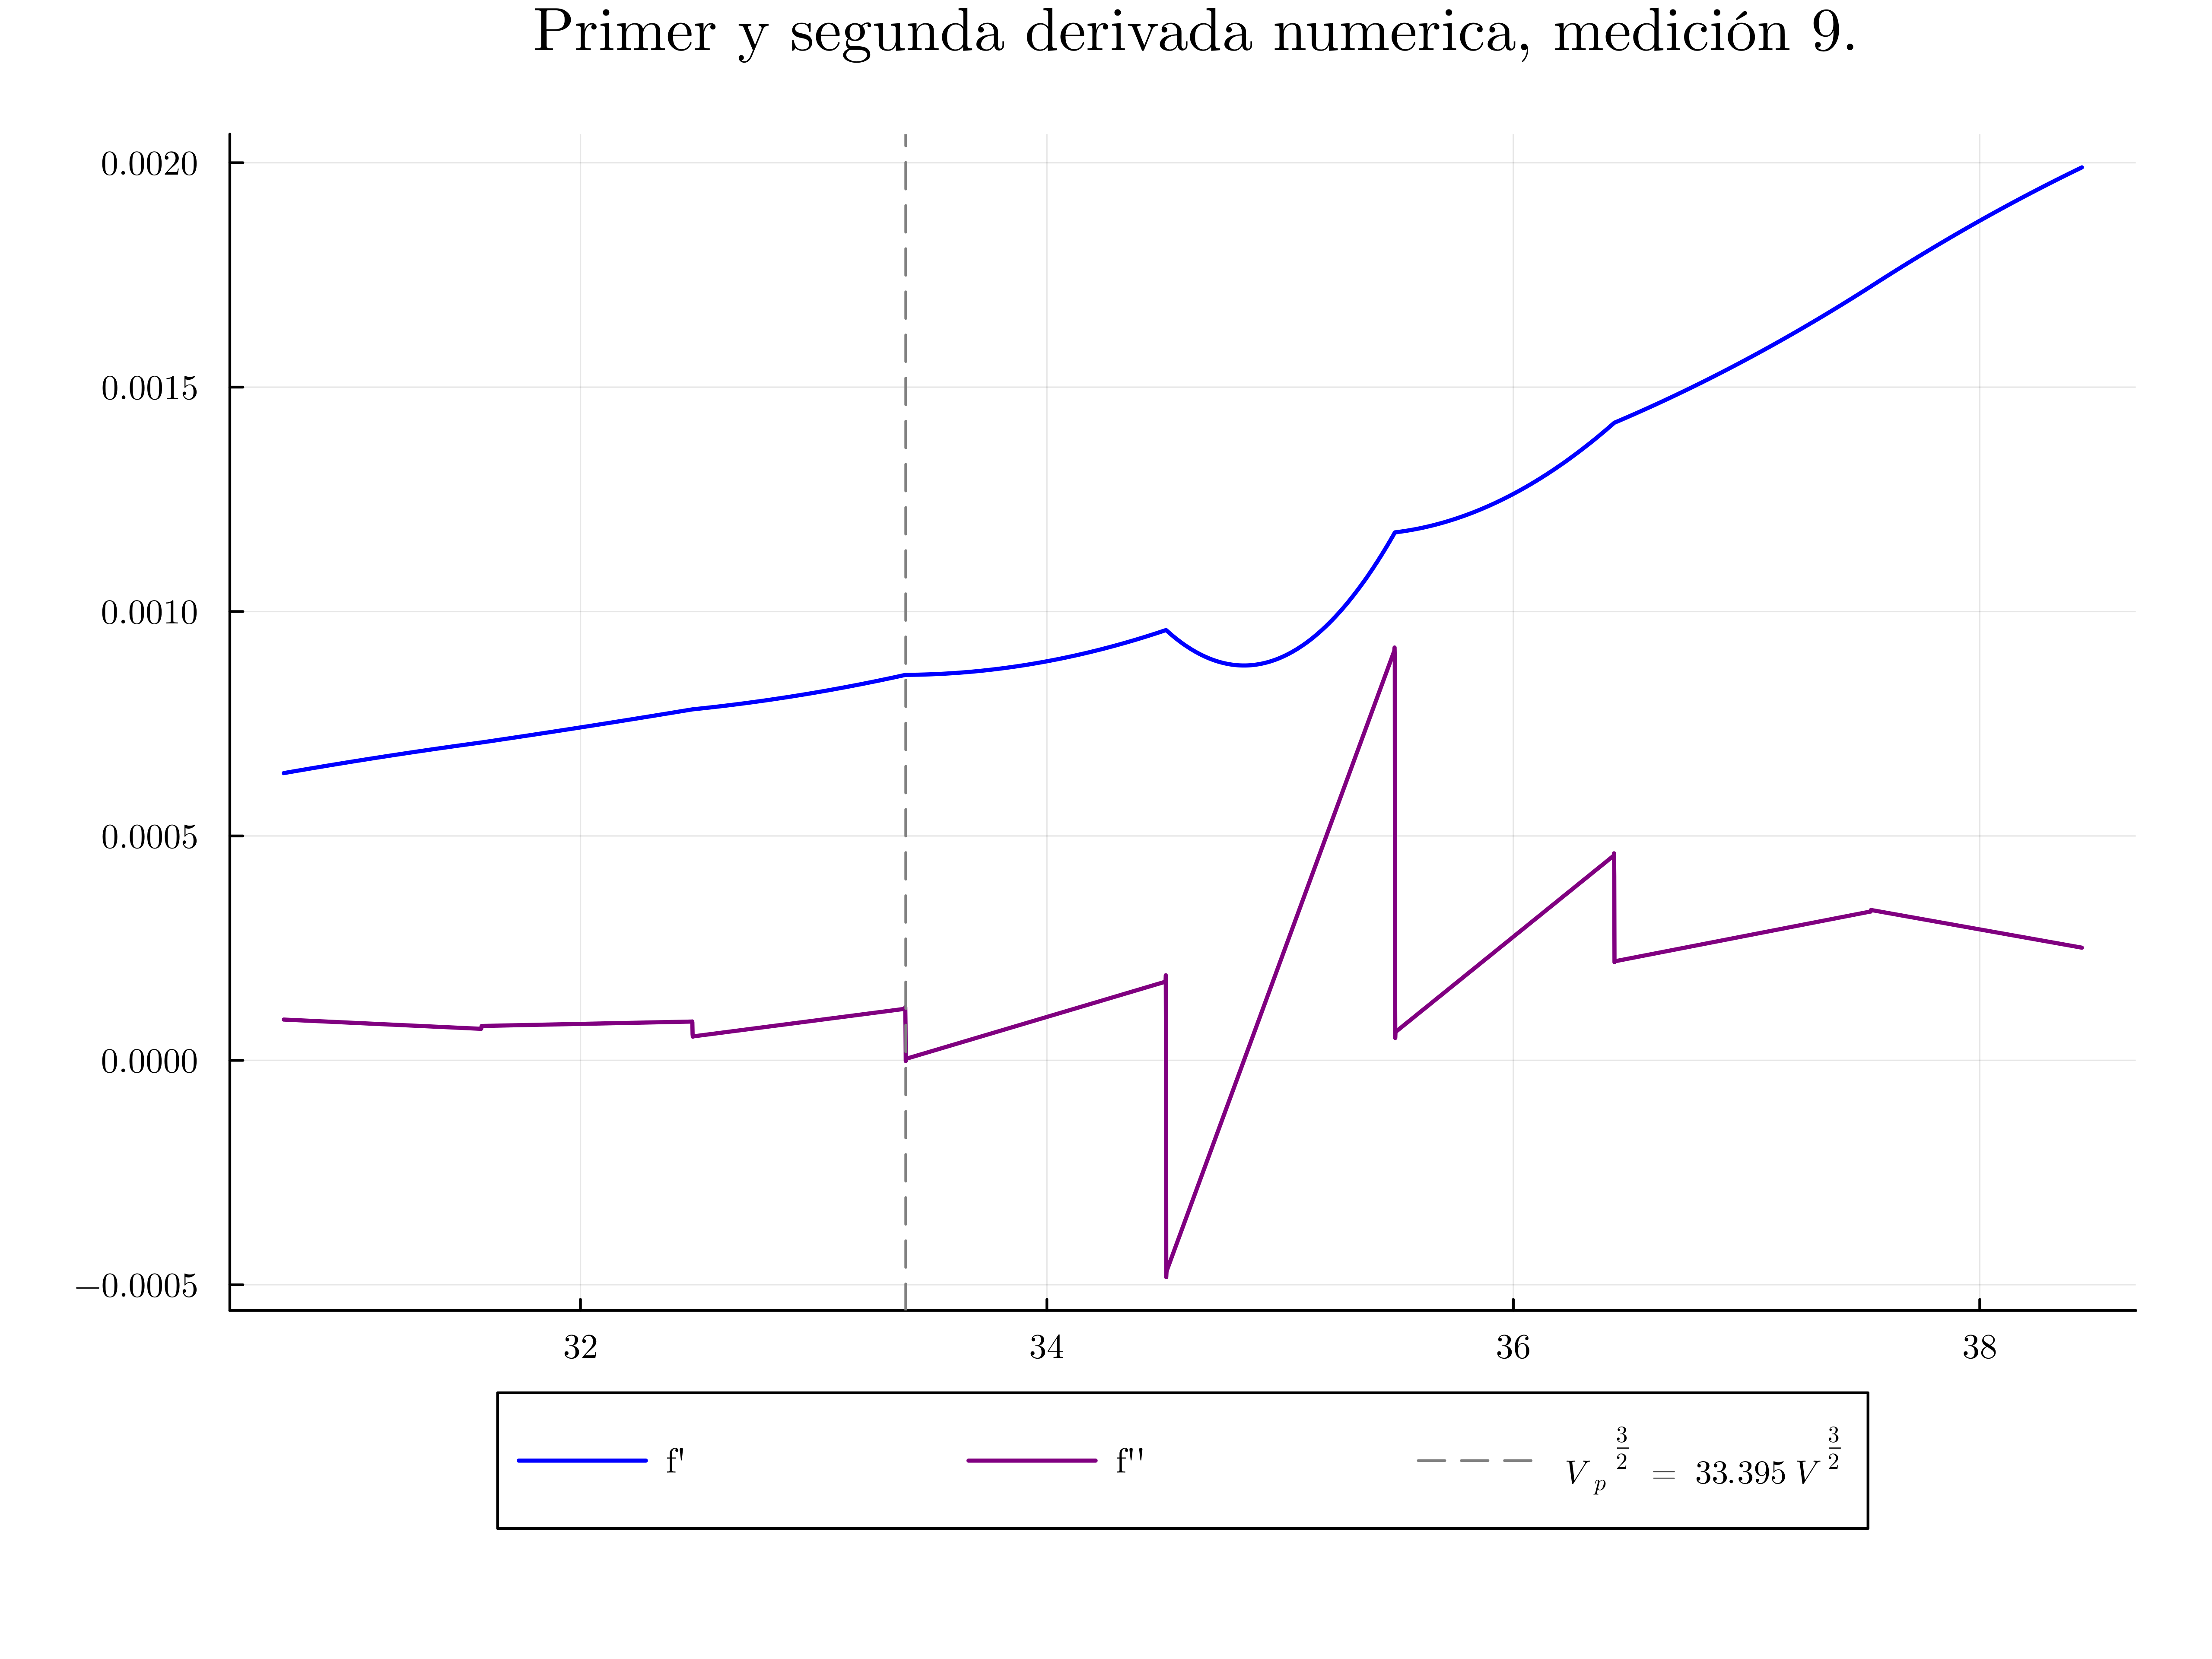
\includegraphics[width=\linewidth]{img/potderps9.png}
	\caption{Barrido n°: 9}
	\label{fig:potderps9}
\end{subfigure}
\hfill
\begin{subfigure}[b]{0.49\textwidth}
	\centering
	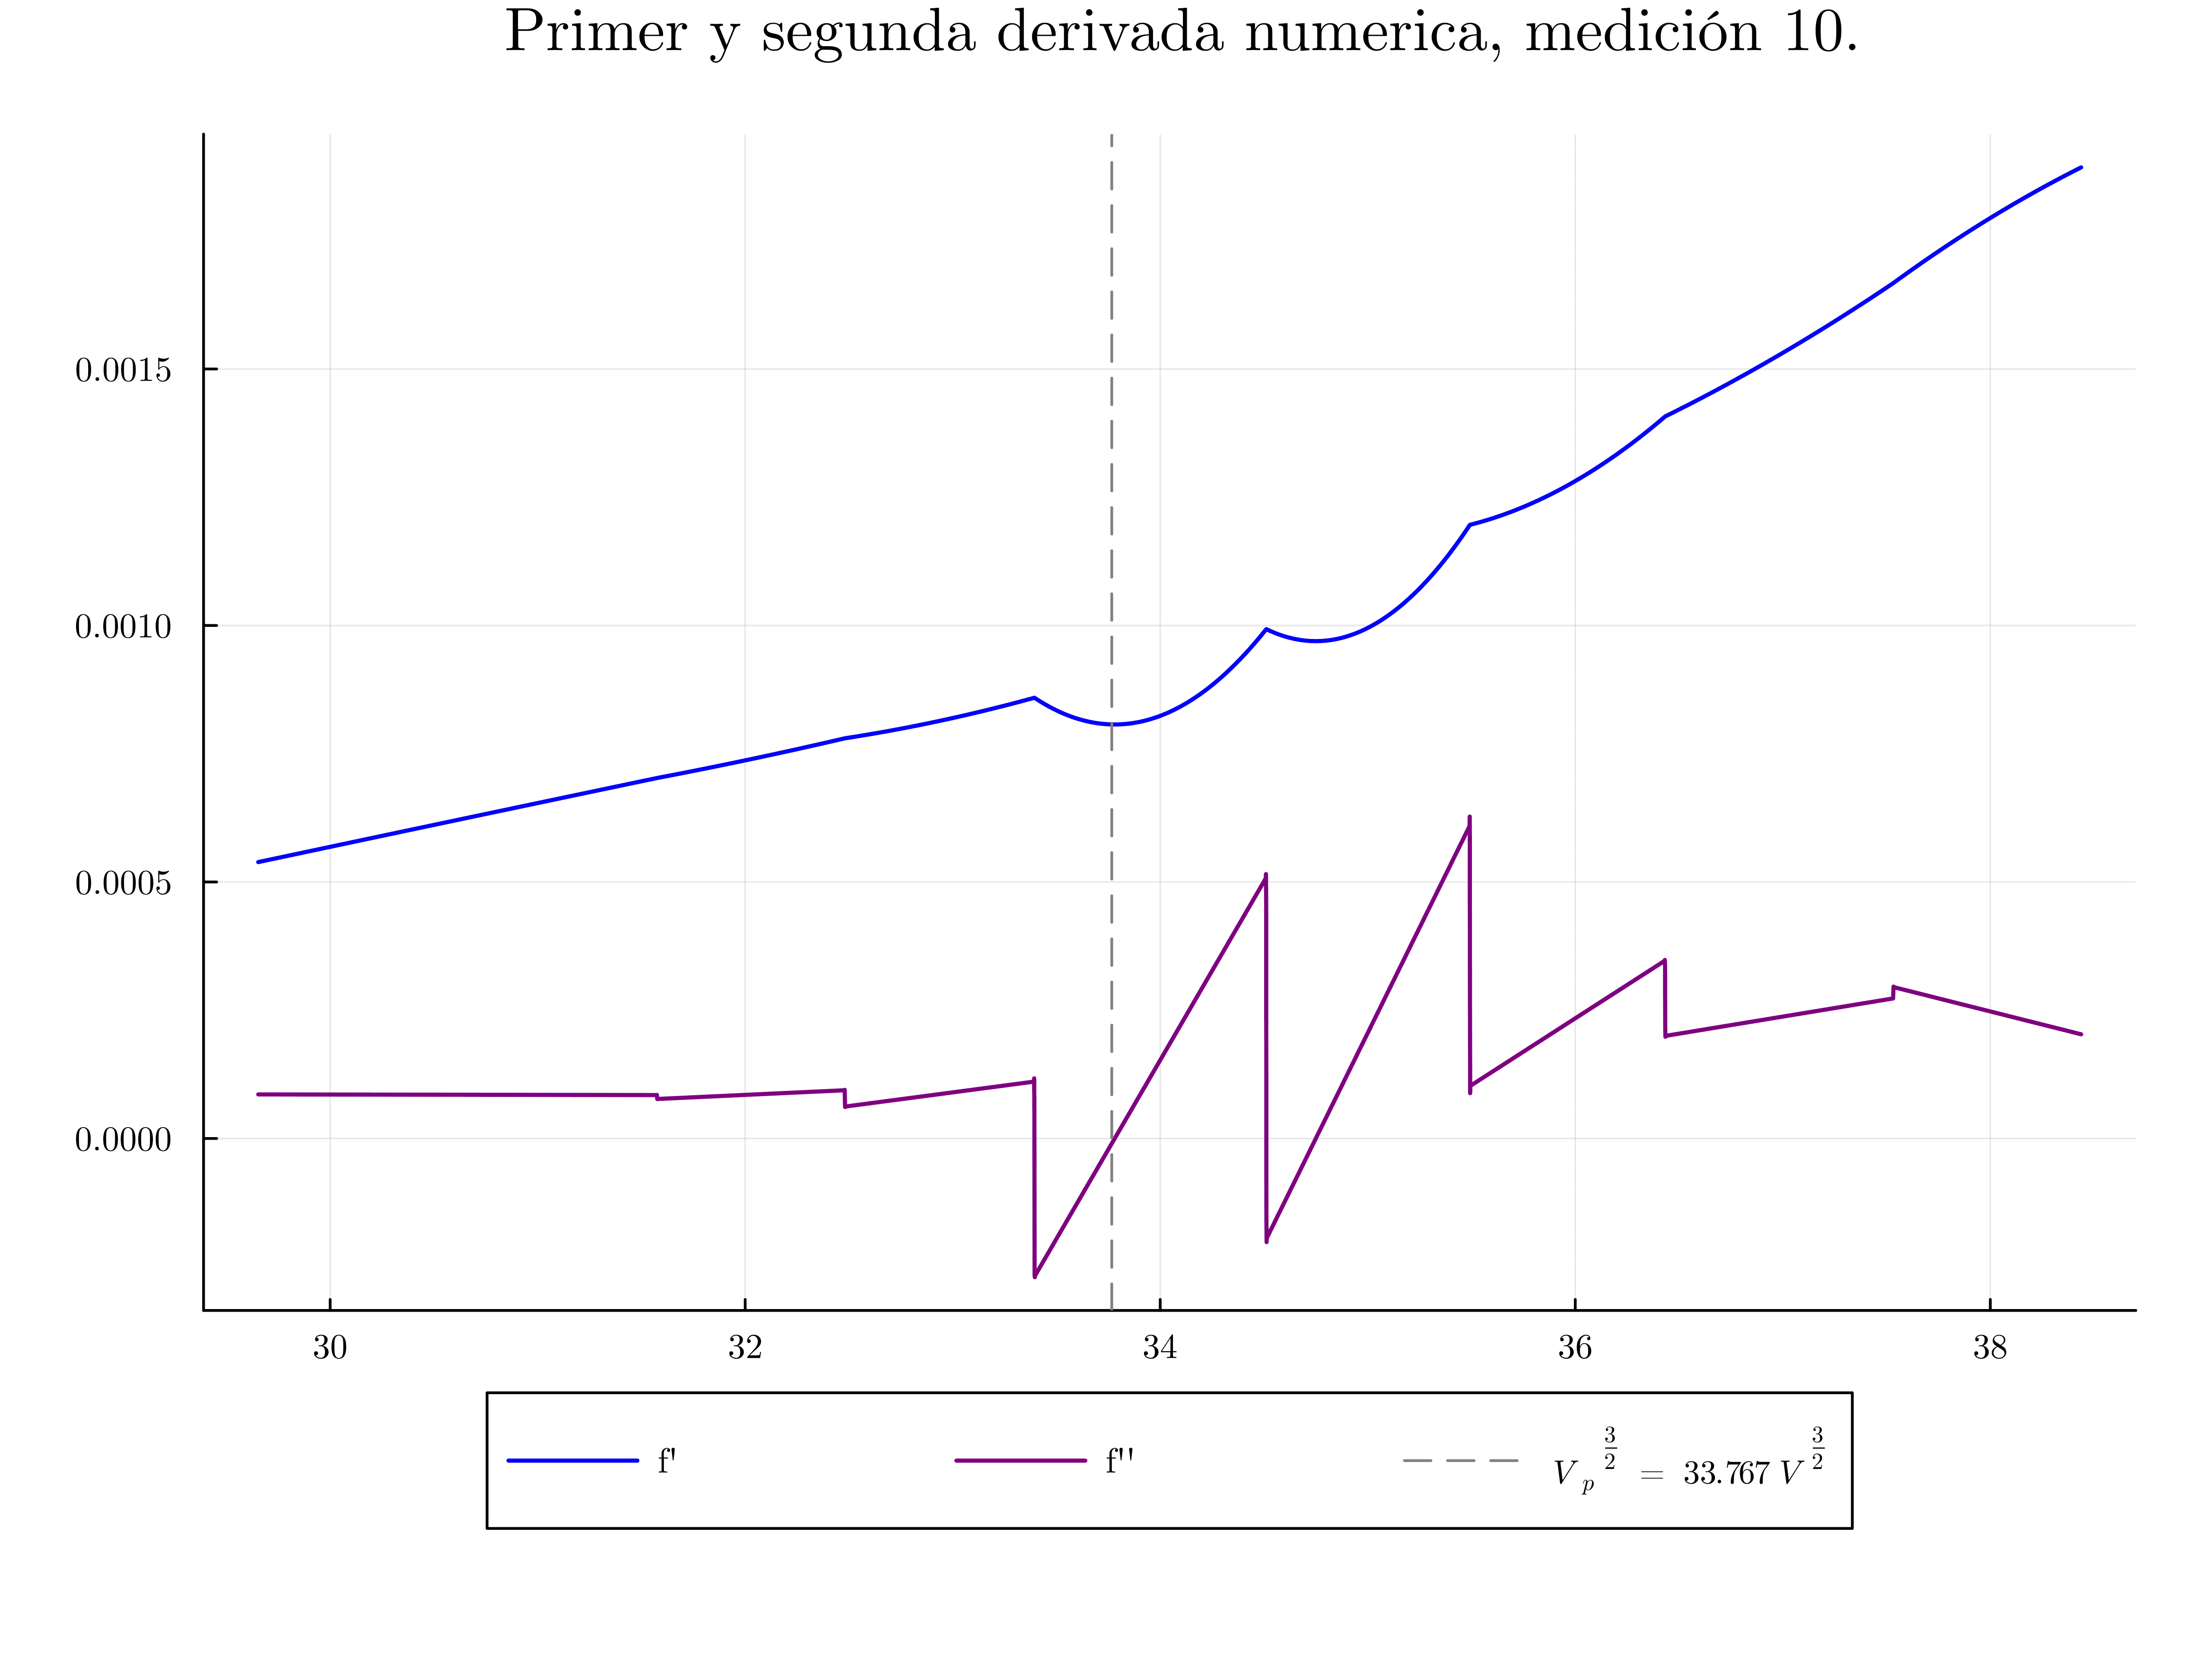
\includegraphics[width=\linewidth]{img/potderps10.png}
	\caption{Barrido n°: 10}
	\label{fig:potderps10}
\end{subfigure}

\caption{Primer y segunda derivada de la corriente del andado con respecto a $V^{\nicefrac{3}{2}}$, para los 10 barridos realizados, donde se puede apreciar la presencia en general de cuatro puntos donde la segunda derivada numérica se acerca a cero, además se puede apreciar que la primera derivada numérica no es suave. Estos fenómenos son causados debido al ruido de la corriente medida el cual se ve trasladado en el algoritmo de LOESS al cambiar en este región múltiples veces de curvatura para ajustar una curva suave, por lo que el punto de inflexión no puede ser detectado de forma gráfica y debe ser determinado mediante el punto en el dominio de $f^{\prime \prime}$ cuyo error con respecto al cero sea menor a $1\times10^{-5}$.}
\label{fig:potderps}
\end{figure}

\twocolumngrid